\documentclass[11pt]{article}

\usepackage[margin=0.75in]{geometry}
\usepackage{amsfonts, amsmath, amssymb}
\usepackage[none]{hyphenat}
\usepackage{fancyhdr}
\usepackage{graphicx}
\usepackage{float}
\usepackage[nottoc, notlot, notlof]{tocbibind}

% circuitikz 
\usepackage[]{circuitikz}

\def\normalcoord(#1){coordinate(#1)}
\def\showcoord(#1){coordinate(#1) node[circle, red, draw, inner sep=1pt,
pin={[red, overlay, inner sep=0.5pt, font=\tiny, pin distance=0.1cm,
pin edge={red, overlay}]45:#1}](){}}
\let\coord=\normalcoord
\let\coord=\showcoord
% circuitikz


\pagestyle{fancy}
\fancyhead{}
\fancyfoot{}
\fancyhead[L]{Electronics (course 25032)}
\fancyhead[R]{Reza Nayeb Habib 401102694}
\fancyfoot[C]{\thepage}
\fancyfoot[R]{Sharif University of Technology}
\renewcommand{\footrulewidth}{1pt}
\parindent 0ex

\begin{document}

    
\begin{titlepage}
\begin{center}

\begin{figure}[H]
\begin{center}

\includegraphics[scale=0.4]{Fig/SUT.png}

\end{center}
\end{figure}

\huge{\textbf{Electronics 2 Project(part 1) Report}} \\ 
\vspace*{2cm}
\Large{\textbf{Instructor: Dr. Medi}} \\
\vspace*{1cm}
\huge{\textbf{Sharif University of Technology}} \\
\line(1,0){500} \\ 
\Huge{\textbf{LM741 Operational Amplifier first stage analysis}} \\
\line(1,0){500} \\
\vfill
\Large{By Reza Nayeb Habib}\\
\Large{Student ID\# 401102694} \\

\end{center}
\end{titlepage}

\tableofcontents
\thispagestyle{empty}
\clearpage
\setcounter{page}{1}

\section{Introduction}
\subsection{Adder and Subtractor} 

\begin{figure}[H]
    \centering
    \resizebox{0.6\textwidth}{!}{%
    \begin{circuitikz}[american]
        \tikzstyle{every node}=[font=\Large]
        \draw (2.5,12.75) node[op amp,scale=1] (opamp2) {};
        \draw (opamp2.+) to[short] (1,12.25);
        \draw  (opamp2.-) to[short] (1,13.25);
        \draw (3.7,12.75) to[short](4,12.75);
        \draw (1,12.25) to (0.5,12.25) node[ground]{};
        \draw (1,13.25) to[short] (-2,13.25);
        \draw (-2,13.25) to[short] (-2,12.5);
        \draw (-2,12.5) to[R] (-2,11);
        \draw (-0.75,13.25) to[short] (-0.75,12.5);
        \draw (-0.75,12.5) to[R] (-0.75,11);
        \draw (0.75,14.5) to[R] (3.5,14.5);
        \draw (0.75,13.25) to[short] (0.75,14.5);
        \draw (3.5,14.5) to[short] (3.5,12.75);
        \draw (4,12.75) to[short, -o] (4.75,12.75);
        \draw (4.75,11) to[short, -o] (4.75,11.75);
        \draw (4.75,11) to (4.75,10.75) node[ground]{};
        \draw (-2,10.25) to[short, o-] (-2,11);
        \draw (-0.75,10.25) to[short, o-] (-0.75,11);
        \node [font=\normalsize] at (5,12.75) {+};
        \node [font=\normalsize] at (5,11.75) {\_};
        \node [font=\normalsize] at (5.5,12.25) {$v_o$};
        \node [font=\normalsize] at (-2,9.75) {$v_i1$};
        \node [font=\normalsize] at (-0.75,9.75) {$v_i2$};
        \node [font=\Large] at (-3.25,11.5) {$R_1$};
        \node [font=\Large] at (0,11.5) {$R_2$};
        \node [font=\Large] at (2,15.25) {$R_3$};
        \end{circuitikz}
        }%

    
    \label{fig:adder}
    \caption{Adder circuit using Op-Amp}
    \end{figure}

    by writing KCL at the inverting node of the amplifier we get:
    $$ v_o = -\frac{R_3}{R_1}v_1 - \frac{R_3}{R_2}v_2 $$

    \begin{figure}[H]
        \centering
        \resizebox{0.6\textwidth}{!}{%
        \begin{circuitikz}[american]
            \tikzstyle{every node}=[font=\Large]
            \draw (-0.5,14.5) node[op amp,scale=1] (opamp2) {};
            \draw (opamp2.+) to[short] (-2,14);
            \draw  (opamp2.-) to[short] (-2,15);
            \draw (0.7,14.5) to[short](1,14.5);
            \draw (-2,15) to[R] (-4.75,15);
            \draw (-3.5,13.75) to[R] (-3.5,11.75);
            \draw (-2,14) to[R] (-2,11.5);
            \draw (-3.5,11) to[short, o-] (-3.5,11.5);
            \draw (-2,11.5) to (-2,11.25) node[ground]{};
            \draw (-4.75,15) to[short, -o] (-5,15);
            \draw (-2,16.5) to[R] (0.75,16.5);
            \draw (2,13) to (2,12.5) node[ground]{};
            \draw (2,13) to[short, -o] (2,13.25);
            \draw (1,14.5) to[short, -o] (2,14.5);
            \draw (-2,14) to[short] (-3.5,14);
            \draw (-3.5,14) to[short] (-3.5,13.5);
            \draw (-3.5,11.75) to[short] (-3.5,11.5);
            \node [font=\normalsize] at (-3.5,10.5) {$v_i1$};
            \node [font=\normalsize] at (-5.75,15) {$v_i2$};
            \node [font=\normalsize] at (3,13.75) {$v_o$};
            \node [font=\normalsize] at (2.5,14.5) {+};
            \node [font=\normalsize] at (2.5,13.25) {\_};
            \draw (-2.25,15) to[short] (-2.25,16.5);
            \draw (-2.25,16.5) to[short] (-2,16.5);
            \draw (0.75,16.5) to[short] (0.75,14.5);
            \node [font=\Large] at (-4.25,12.75) {$R_1$};
            \node [font=\Large] at (-3.5,15.75) {$R_2$};
            \node [font=\Large] at (-2.5,12.75) {$R_3$};
            \node [font=\Large] at (-0.5,17.25) {$R_4$};
            \end{circuitikz}
            }%
    
        
        \label{fig:subtractor}
        \caption{Subtractor circuit using Op-Amp}  
\end{figure}

again by writing KCL at the inverting node of the amplifier and also 
knowing that the inverting and non-inverting node of the amplifier have the same voltage
we get:
$$ v_o = \frac{R_3}{R_4(R_1+R_3)}v_1 - \frac{R_4}{R_2}v_2 $$

\subsection{Log of a signal}
\begin{figure}[H]
    \centering
    \resizebox{0.6\textwidth}{!}{%
    \begin{circuitikz}[american]
        \tikzstyle{every node}=[font=\large]
        \draw (-0.75,14.75) node[op amp,scale=1] (opamp2) {};
        \draw (opamp2.+) to[short] (-2.25,14.25);
        \draw  (opamp2.-) to[short] (-2.25,15.25);
        \draw (0.45,14.75) to[short](0.75,14.75);
        \draw (-2.25,14.25) to (-3,14.25) node[ground]{};
        \draw (-4,15.25) to[short, -o] (-4.5,15.25);
        \draw (-2,16.5) to[short] (-2,15.25);
        \draw (0.25,16.5) to[short] (0.75,16.5);
        \draw (0.75,16.5) to[short] (0.75,14.75);
        \draw (0.75,14.75) to[short] (1.75,14.75);
        \draw (1.75,14.75) to[short, -o] (2,14.75);
        \draw (2,12.75) to[short, -o] (2,13.5);
        \draw (2,12.75) to (2,12.25) node[ground]{};
        \node [font=\normalsize] at (-5.25,15.25) {$v_i$};
        \node [font=\normalsize] at (2.5,13.5) {-};
        \node [font=\normalsize] at (2.5,14.75) {+};
        \node [font=\normalsize] at (3,14.25) {$v_o$};
        \node [font=\large] at (6,17.5) {};
        \draw (-4,15.25) to[R] (-2.25,15.25);
        \draw (-2,16.5) to[D] (0.25,16.5);
        \node [font=\large] at (-3.25,16) {R};
        \end{circuitikz}
        }%

    
    \label{fig:signalLogCalculator}
    \caption{Signal log calculator circuit using Op-Amp}  
\end{figure}
$$ i_D = \frac{v_i}{R} $$
$$ v_o = -v_Tln(\frac{v_i}{RI_s}) $$


\subsection{square and triangle wave generator}
\begin{figure}[H]
    \begin{center}
        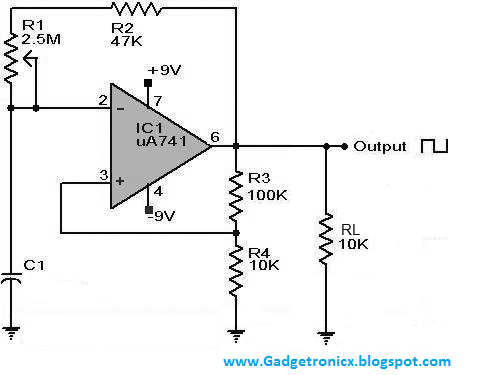
\includegraphics[scale=0.5]{Fig/square.png}
        \label{fig:square}
        \caption{square wave generator using op-amp}
    \end{center}
\end{figure}
Let us assume the voltage at inverting terminal be V2 which equals to the voltage across the capacitor. Also, let us assume the voltage at the non-inverting terminal be V1. The voltage difference between non-inverting and inverting terminal is referred to as differential input voltage and is given by Vin. \\
At the initial state when the capacitor is fully discharged, the voltage at inverting pin will be zero, i.e. V2 = 0V \\
Therefore, input differential voltage (Vin) = V1-V2 = V1-0 = V1 \\
When Vin is positive the output is also positive, at this instance, the capacitor starts to charge through resistor R2 towards positive saturation voltage until V1 = V2. \\
When the voltage at the capacitor increases slightly more than the differential voltage V1. \\
Negative Vin = V1-V2 (V2 $>$ V1) \\
Then the output will be switched from positive saturation voltage to negative saturation voltage. In this instance, the capacitor starts to discharge through resistor R2 because V2 becomes greater than Vout. Again, after reaching V2 slightly less than V1 the output will again switch to positive saturation voltage. This process repeats again and again as a result square wave is generated. \\ \\
we can easily combine this circuit with an integrator to get a triangular circuit like below figure:

\begin{figure}[H]
    \begin{center}
        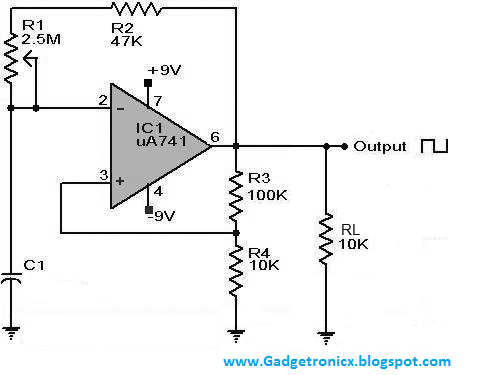
\includegraphics[scale=0.5]{Fig/square.png}
        \label{fig:square}
        \caption{square wave generator using op-amp}
    \end{center}
\end{figure}

\subsection{square and triangle wave generator}
\begin{figure}[H]
    \begin{center}
        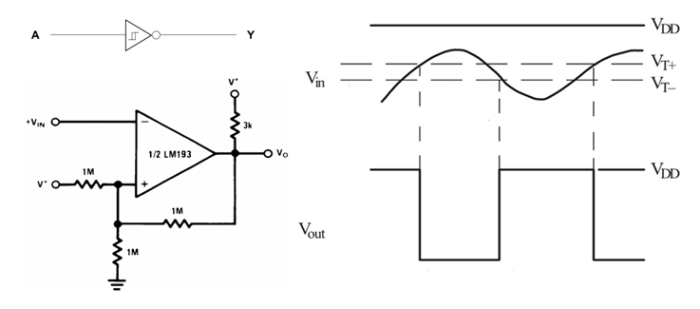
\includegraphics[scale=0.5]{Fig/schmitt.png}
        \label{fig:schmitt}
        \caption{shmitt trigger using op-amp}
    \end{center}
\end{figure}

\begin{figure}[H]
    \begin{center}
        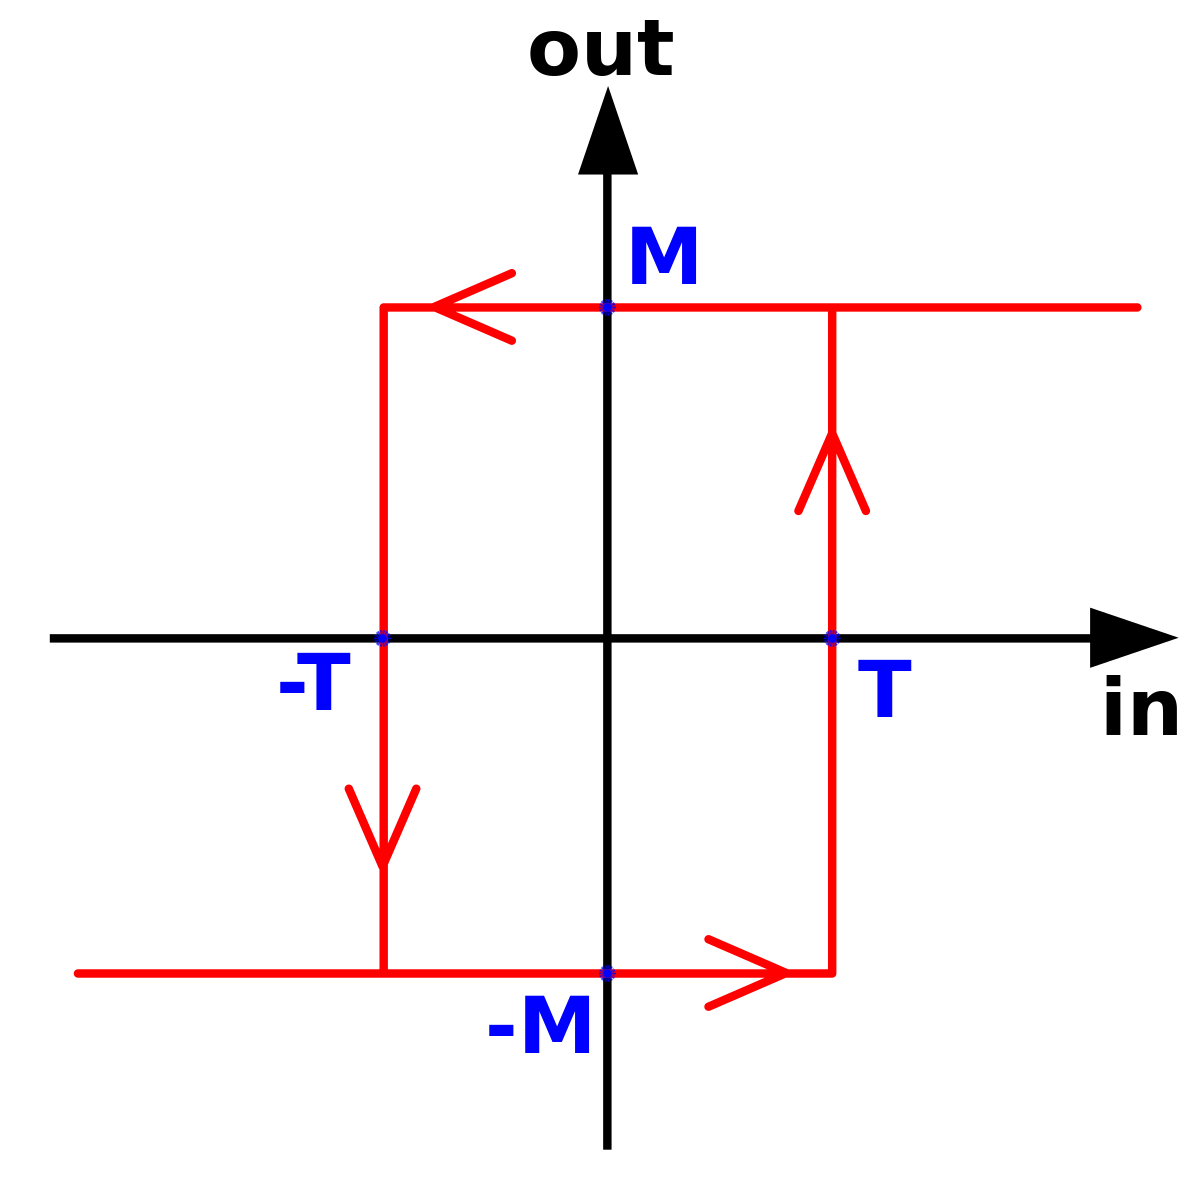
\includegraphics[scale=0.1]{Fig/schmitt-characteristic.png}
        \label{fig:schmitt trigger characterisitcs}
        \caption{shmitt trigger characterisitc}
    \end{center}
\end{figure}
shmitt trigger uses feedback to compare our input to some voltage $\pm V$ and drop to $-V_{cc}$ when our voltage
gets more than V and get to $-V_{cc}$ when the voltage gets less than -V. this circuit has a hysteresis characterisitc.




\section{LM741 IC characterisitcs}
\subsection*{a)}
\begin{figure}[H]
    \begin{center}
        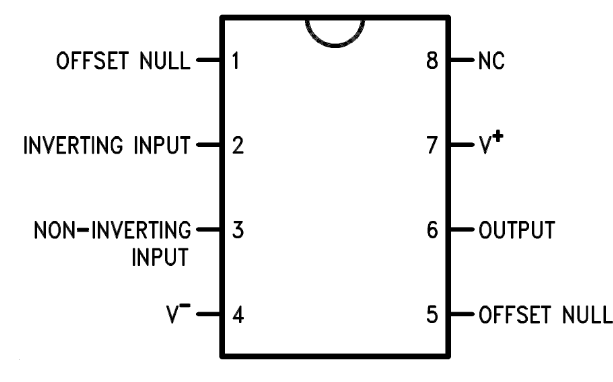
\includegraphics[scale=0.5]{Fig/LM741-IC.png}
        \label{fig:lm741IC}
        \caption{the LM741 IC ports}
    \end{center}
\end{figure}
as it can be seen in the Figure above ports 2 and 3 are the non-inverting and inverting
input ports. port 7 and 4 are the ports that we connect Vcc and Vee. and port 6 is the output port.
also ports 1 and 5 are for offset null by wich we remove the output unwanted DC value.
\subsection*{b)}
this op-amp works with supply voltage $\pm22V$ and also can get differential input voltage up to $\pm30V$. \\
it also uses $60mW$ to $150mW$ of power depending on the amplifier type and can work in temperatures of $-55^\circ \mathrm{C}$ to $125^\circ \mathrm{C}$
\subsection*{c)}
the large signal voltage gain can vary betwenn 20,000 and 200,000. and the input current drift is about 0.5 nA.
the input resistance can vary between 300k$\Omega$ to 6M$\Omega$ in different models and different bias points. \\
the CMRR can vary between 70dB to 95dB.\\
the circuit can swing $\pm16V$ and the typical power consumption is about $100mW$.

\section{Designing an amplifier circuit}
\subsection{analyze the different parts of this circuit}
\begin{figure}[H]
    \begin{center}
        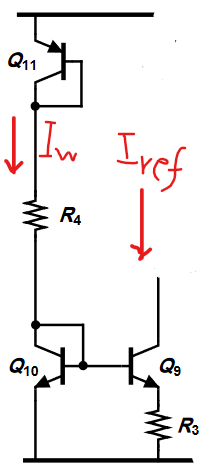
\includegraphics[scale=0.7]{Fig/widlar.png}
        \label{fig:widlar}
        \caption{the widlar part of the circuit}
    \end{center}
\end{figure}
we can see that this part of the circuit is a Widlar current source.
we derive $I_w$ and $I_{ref}$ here to use them later in synthesis section:
$$ I_w = \frac{28.6}{R_4} $$
$$ I_{ref}R_3 = v_Tln(\frac{I_w}{I_{ref}}) $$


\begin{figure}[H]
    \begin{center}
        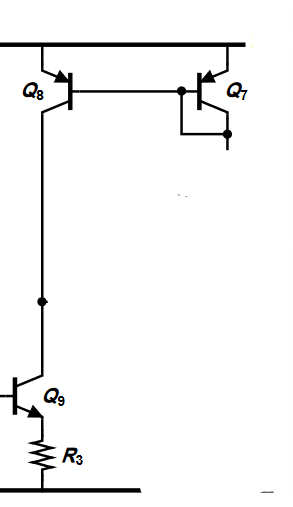
\includegraphics[scale=0.7]{Fig/mirror.png}
        \label{fig:mirror}
        \caption{the current mirror for copying $I_{ref}$}
    \end{center}
\end{figure}

this part only copies $I_{ref}$ to our amplifying section.

\begin{figure}[H]
    \begin{center}
        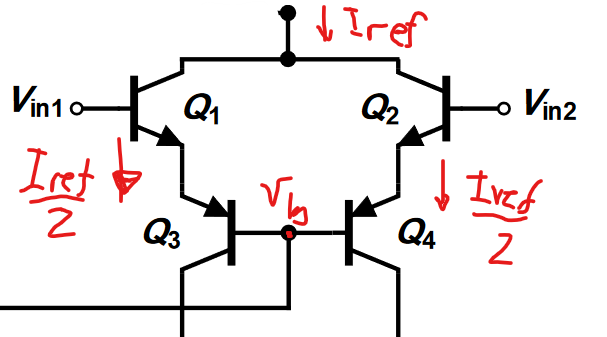
\includegraphics[scale=0.7]{Fig/signalInput.png}
        \label{fig:inputSignal}
        \caption{signal input part of the amplifier}
    \end{center}
\end{figure}
first we should point that $Q_1$, $Q_2$, $Q_3$, $Q_4$, $Q_5$, $Q_6$
all have the same $ I_C = \frac{I_{ref}}{2} $ so they all have the same $g_m$ and $r_e$. \\ \\


\begin{figure}[H]
    \begin{center}
        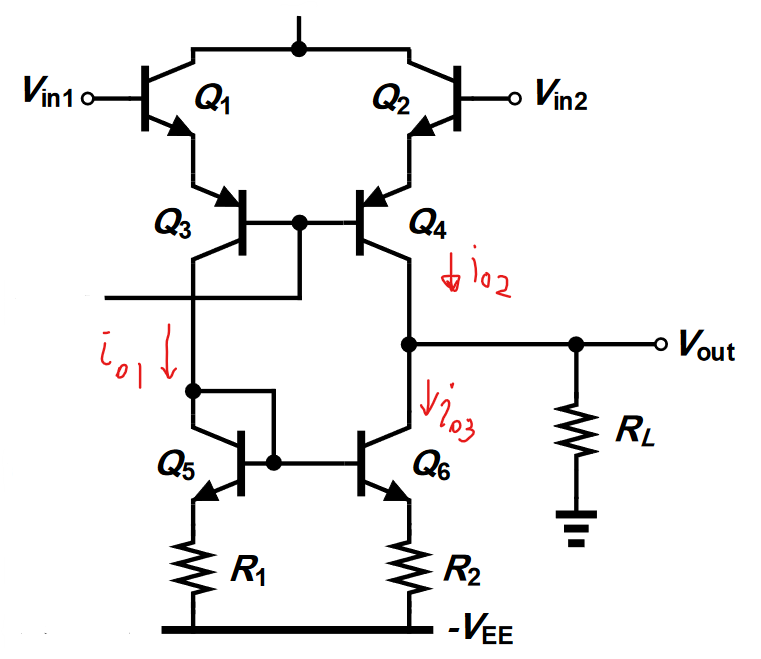
\includegraphics[scale=0.7]{Fig/smallSigCircuit.png}
        \label{fig:smallSignalCircuit}
        \caption{the currents marked on this circuits will be used for calculating the gain}
    \end{center}
\end{figure}
we now start the small signal analysis of 
now assuming that the input is differential we can consider $v_b$ as GND in small signal. \\
we can then use the t model for transistors to anlyze this parts half circuits:
\begin{figure}[H]
    \centering
    \resizebox{0.4\textwidth}{!}{%
    \begin{circuitikz}[american]
        \tikzstyle{every node}=[font=\large]
        \draw (-6,13.75) to[short, -o] (-7,13.75);
        \draw (-6,15.75) to[american controlled current source] (-6,13.75);
        \draw (-4.75,15.75) to[R] (-4.75,13.75);
        \draw (-6,13.75) to[R] (-6,11.75);
        \draw (-6,11.75) to[R] (-6,10);
        \draw (-6,10) to (-6.75,10) node[sground]{};
        \draw (-6,10) to[american controlled current source] (-6,7.75);
        \draw (-4.75,10) to[R] (-4.75,7.75);
        \draw (-6,10) to[short] (-4.75,10);
        \draw (-6,7.75) to[short] (-4.75,7.75);
        \draw (-6,7.75) to[short] (-6,7);
        \draw (-6,15.75) to[short] (-4.75,15.75);
        \draw (-6,13.75) to[short] (-4.75,13.75);
        \node [font=\large] at (-7.5,13.75) {$v_{in1}$};
        \node [font=\large] at (-5,12.75) {$v_{e1}$};
        \node [font=\large] at (-5,11) {$v_{e3}$};
        \node [font=\large] at (-5.25,11.5) {+};
        \node [font=\large] at (-5.25,10.25) {\_};
        \node [font=\large] at (-5.25,13.25) {+};
        \node [font=\large] at (-5.25,12) {\_};
        \draw (-6,13.75) to[short] (-4.75,13.75);
        \node [font=\large] at (-7,12.75) {$r_{e1}$};
        \node [font=\large] at (-7,11) {$r_{e3}$};
        \node [font=\large] at (-3.75,14.75) {$r_{o1}$};
        \node [font=\large] at (-3.75,9) {$r_{o3}$};
        \node [font=\large] at (-7.25,14.75) {$g_{m1}v_{e1}$};
        \node [font=\large] at (-7.25,8.75) {$g_{m3}v_{e3}$};
        \draw [ color={rgb,255:red,255; green,0; blue,0}, line width=0.7pt, ->, >=Stealth] (-6.5,7.75) -- (-6.5,6.25);
        \node [font=\large, color={rgb,255:red,255; green,0; blue,0}] at (-7.25,7.25) {$i_{o1}$};
        \end{circuitikz}
        }%
    \label{fig:inputSmallSig}
    \caption{Small signal model of $Q_1$ and $Q_3$(same as $Q_2$ and $Q_4$ due to symmetry)}  
\end{figure}
*[firstly pay attention that we are going to calculate $G_m$ for this circuit and then multiply it by
$R_L$ so remember in all of the steps below the output is assumed short circuit(meaning $R_L = 0$)]\\ \\
in the above figure we can see:
$$ v_{e3} = \frac{r_{e3}}{r_{e3} + r_{e1}}v_{in1} = \frac{1}{2}v_{in} $$ 
assuming the resistance in $i_{o1}$ being sufficiently small (it can be achieved by choosing an $R_1$ smaller than $r_{o3}$) we can say that:
$$ i_{o1} = \frac{1}{2}g_{m3}v_{in1} $$
because the output is shorted we can also write:
$$ i_{o2} = \frac{1}{2}g_{m4}v_{in2} = -\frac{1}{2}g_{m4}v_{in1} $$
also we can easily see that the input impedance is:
$$ R_{in} = 2\beta_n(r_{e1} + r_{e3}) = 4\beta_n(r_{e1}) = 8\beta_n\frac{v_T}{I_{ref}} $$

now $Q_5$ and $Q_6$ form a current mirror for copying $i_{o1}$ into $i_{o3}$ their small signal form is:
\begin{figure}[H]
    \centering
    \resizebox{0.4\textwidth}{!}{%
    \begin{circuitikz}[american]
        \tikzstyle{every node}=[font=\LARGE]
        \draw (4.75,11) to[R=$r_{e5}$] (4.75,9);
        \draw (4.75,9) to[R=$R_1$] (4.75,7);
        \draw (6.75,8.75) to[R=$R_2$] (6.75,7.25);

        \draw (4.75,11) to[short] (6.75,11);

        \draw (6.75,10.75) to[R=$r_{e6}$] (6.75,9.25);
        \draw (6.75,13) to[american controlled current source] (6.75,11.25);
        \draw (8,13) to[R=$r_{o6}$] (8,11.25);
        \draw (4.75,7) to (4.75,6.75) node[sground]{};
        \draw (6.75,7.25) to (6.75,6.75) node[sground]{};
        \draw (6.75,8.75) to[short] (6.75,9.25);
        \draw (6.75,10.75) to[short] (6.75,11.25);
        \draw (6.75,11.25) to[short] (8,11.25);
        \draw (6.75,13) to[short] (8,13);
        \draw (6.75,13) to[short] (6.75,14);
        \node [font=\LARGE] at (7.25,9.5) {\_};
        \node [font=\LARGE] at (7.25,10.75) {+};
        \node [font=\LARGE] at (8.25,10) {$v_{e6}$};
        \node [font=\LARGE] at (5.5,12.25) {$g_{m6}v_{e6}$};
        \draw [ color={rgb,255:red,255; green,0; blue,0}, ->, >=Stealth] (3.5,13) -- (3.5,11.75);
        \draw [ color={rgb,255:red,255; green,0; blue,0}, ->, >=Stealth] (8,14.25) -- (8,13.25);
        \node [font=\LARGE, color={rgb,255:red,255; green,0; blue,0}] at (3,12.75) {$i_{o1}$};
        \node [font=\LARGE, color={rgb,255:red,255; green,0; blue,0}] at (9,13.75) {$i_{o3}$};
        \end{circuitikz}
        }%
    \label{fig:smallSigMirror}
    \caption{Small signal model of $Q_5$ and $Q_6$ currnet mirror}  
\end{figure}
first because output is shorted all of $g_{m6}v_{e6}$ goes to $i_{o3}$.
now we calculate $i_{o3}$:
$$ v_{e6} = i_{o1}\frac{r_{e6}(r_{e5} + R_1)}{r_{e6} + R_2} $$
$$ i_{o3} = i_{o1}\frac{r_{e5} + R_1}{r_{e6} + R_2} = \frac{1}{2}g_{m3}\frac{(r_{e5} + R_1)}{r_{e5} + R_2}v_{in1}$$

now we calculate $i_{out}$:
$$ i_{out} = i_{o2} - i_{o3} = -\frac{1}{2}g_{m4}v_{in1} - \frac{1}{2}g_{m3}\frac{(r_{e5} + R_1)}{r_{e5} + R_2}v_{in1}$$
knowing all $g_m$ and $r_e$ are equal:
$$ G_m = \frac{i_{out}}{2v_{in1}} =  -\frac{1}{4}g_m\frac{2r_e + R_1 + R_2}{r_e + R_2} $$
we then calculate the output impedance:
$$ R_{out} = ( (1+g_m r_{o4})(r_e||r_{\pi4}) )||( (1+g_m r_{o6})(R_2||r_{\pi4}) ) \simeq (g_m r_{o4} r_e) || (g_m r_{o6}(R_2||r_{\pi4}))$$
then the final gain is:
$$ A_v = G_m(R_L||R_{out}) = -\frac{1}{4}g_m\frac{2r_e + R_1 + R_2}{r_e + R_2}(R_L||R_{out}) $$
if we set $R_1 = R_2$ we get: $$ A_v =  -\frac{1}{2}g_m(R_L||R_{out}) $$
and setting $R_1 = R_2$ will increase our common mode rejection but we may or may not do that based on application.
we in particular choose to set them equal. \\

\subsection{choosing theoritical values for the amplifier}
the input impedance as calculated before is:
$$ R_{in} = 8\beta_n\frac{v_T}{I_{ref}} > 2M\Omega \rightarrow I_{ref} < 20\mu A$$
then bounding the gain we have:
$$ A_v = -\frac{1}{2}g_m(R_L||R_{out}) \simeq -\frac{1}{4}\frac{I_{ref}}{v_T}R_L > 316  \rightarrow I_{ref} > 31.6\mu A$$
we can see that there is no $I_{ref}$ fitting both conditions thus we choose the $I_{ref}$ giving
maximum gain with resistance of $2M\Omega$ meaning $I_{ref} = 20\mu A$ wich gives $A_v = 200$. \\ \\

now we find the widlar current in way not to consume more than $400mW$:
$$ I_w = \frac{28.6}{R_4} $$
$$ I_{ref}R_3 = v_Tln(\frac{I_w}{I_{ref}}) \rightarrow R_3 = 3k\Omega \space I_w = 0.2mA$$
we had freedom in choosing $I_w$ and $R_3$ but we chose according to maximum power and also not using very high resistances.
now for $I_w = 0.2mA$ we should set $R_4 = 143k\Omega$.
the choice for $R_1$ and $R_2$ pretty much doesn't limit anything so we choose 1.5k$\Omega$ for them being near the datasheet.
\subsection{Operating point simulation}
\begin{table}[H]
    \begin{tabular}{lllllll}
    Transistor & Ic      & $g_m$     & $r_\pi$ & $V_{CE}$  & $r_o$      \\
    Q1         & 12.75µ  & 510µ   & 392.16k & 15V & 15.69M  \\
    Q2         & 12.75µ  & 510µ   & 392.16k & 15V & 15.69M  \\
    Q3         & -12.75µ & 510µ   & 196.08k & 13.8V & 3.92M   \\
    Q4         & -12.75µ & 510µ   & 196.08k & 1.1V & 3.92M   \\
    Q5         & 12.56µ  & 502.4  & 398.09k & 601mV & 15.92M  \\
    Q6         & 13.5µ   & 540µ   & 370.37k & 13.3V & 14.81M  \\
    Q7         & -24µ    & 960µ   & 104.17k & 590mV & 2.08M   \\
    Q8         & -31.3µ  & 1.25m  & 79.87k  & 16.2V & 1.6M    \\
    Q9         & 31.2µ   & 1.25m  & 160.26k & 13.8V & 6.41M   \\
    Q10        & 180µ    & 7.2m   & 27.78k  & 671mV & 1.11M   \\
    Q11        & -180µ   & 7.2m   & 13.89k  & 642.5mV & 277.78k
    \end{tabular}
\end{table}
\begin{figure}[H]
    \begin{center}
        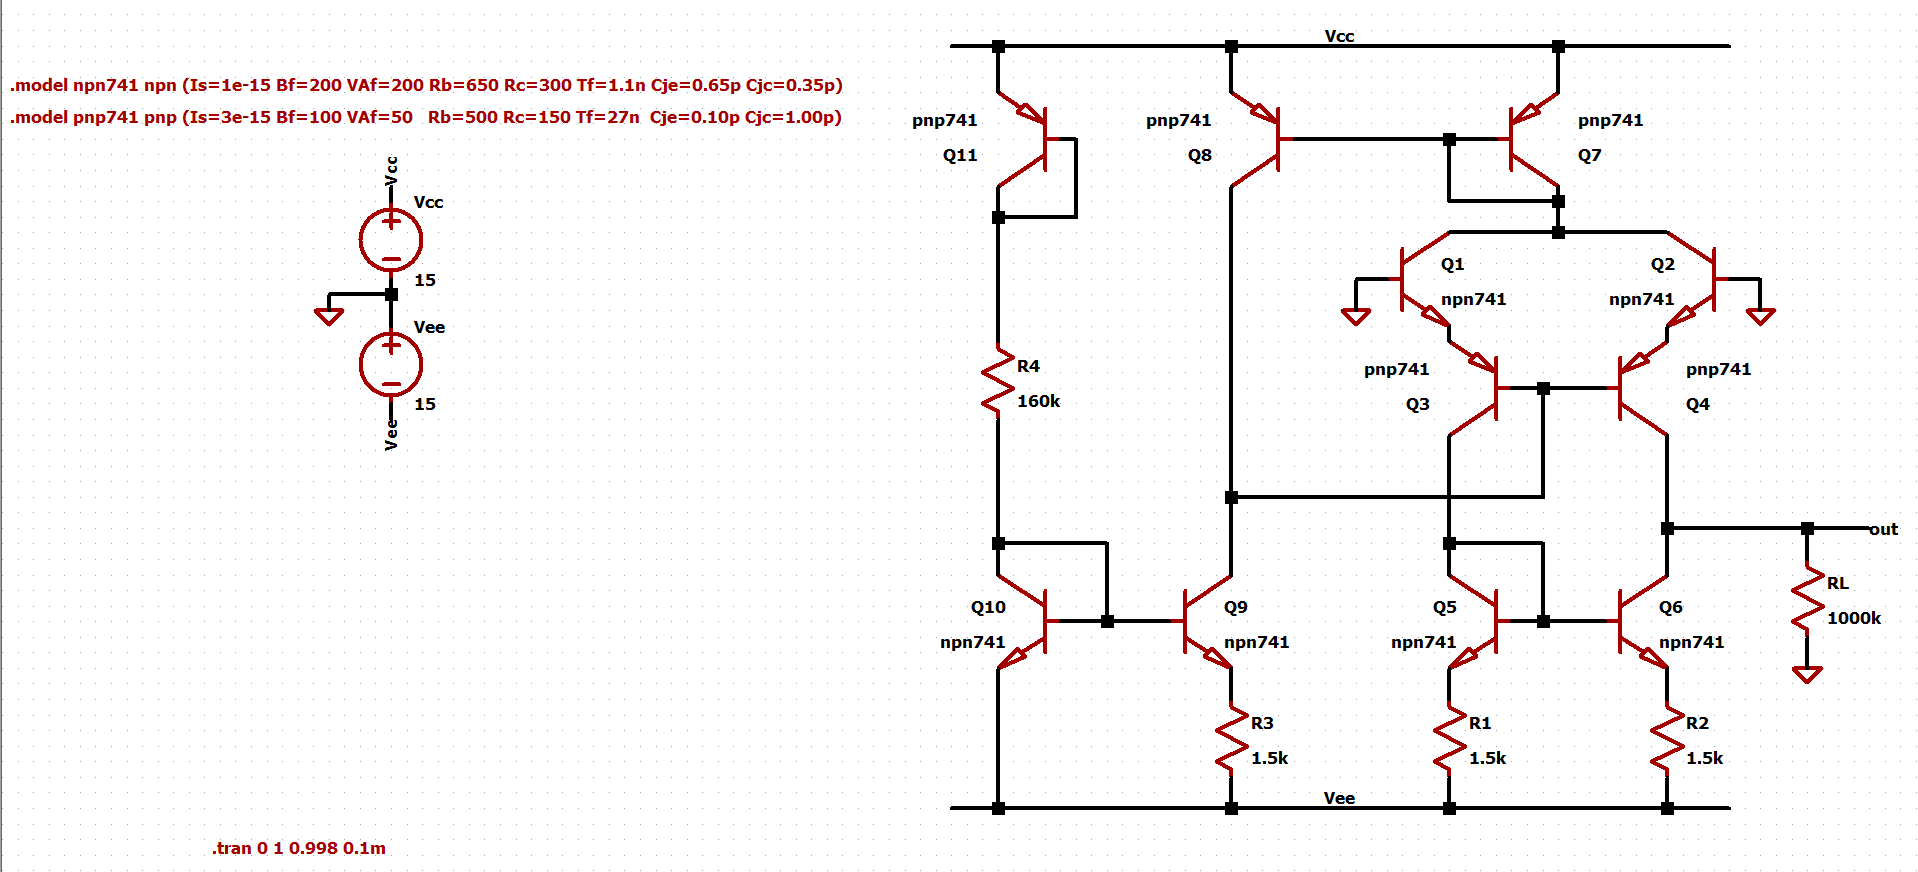
\includegraphics[scale=0.4]{Fig/dc-circuit.png}
        \label{fig:dcCircuit}
        \caption{the DC circuit in ltspice}
    \end{center}
\end{figure}

\subsection{AC analysis simulation}
\begin{figure}[H]
    \begin{center}
        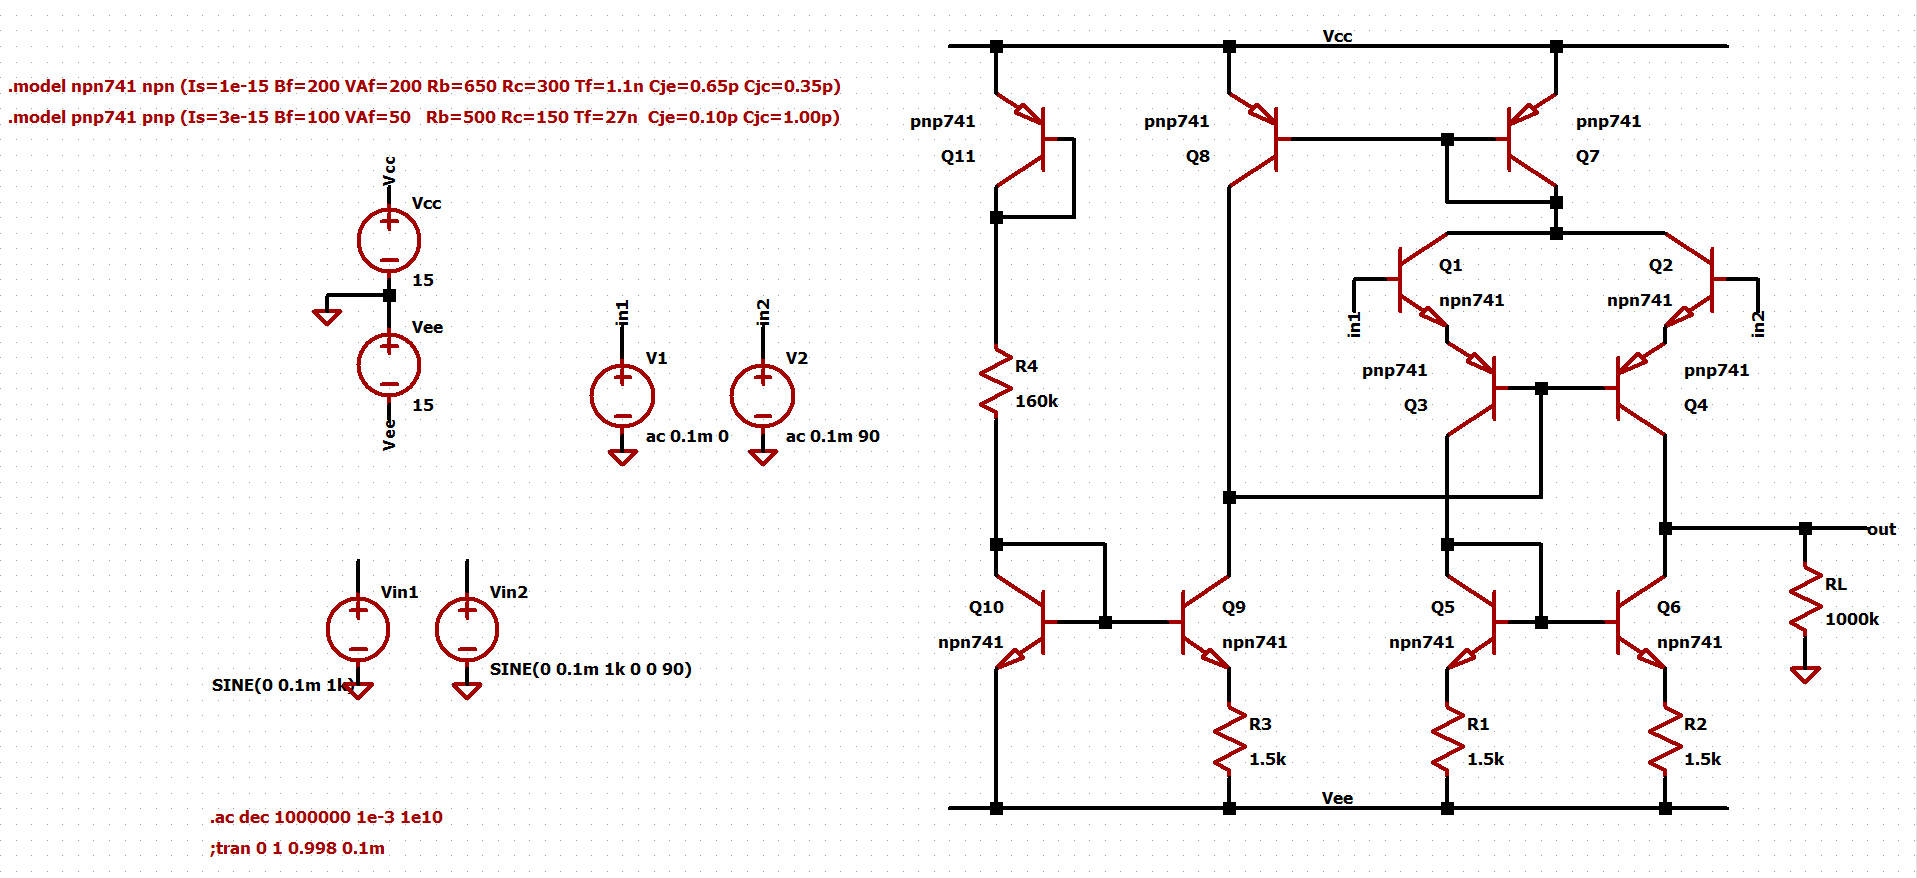
\includegraphics[scale=0.4]{Fig/ac-circuit.png}
        \label{fig:ACCircuit}
        \caption{the AC circuit in ltspice}
    \end{center}
\end{figure}

\begin{figure}[H]
    \begin{center}
        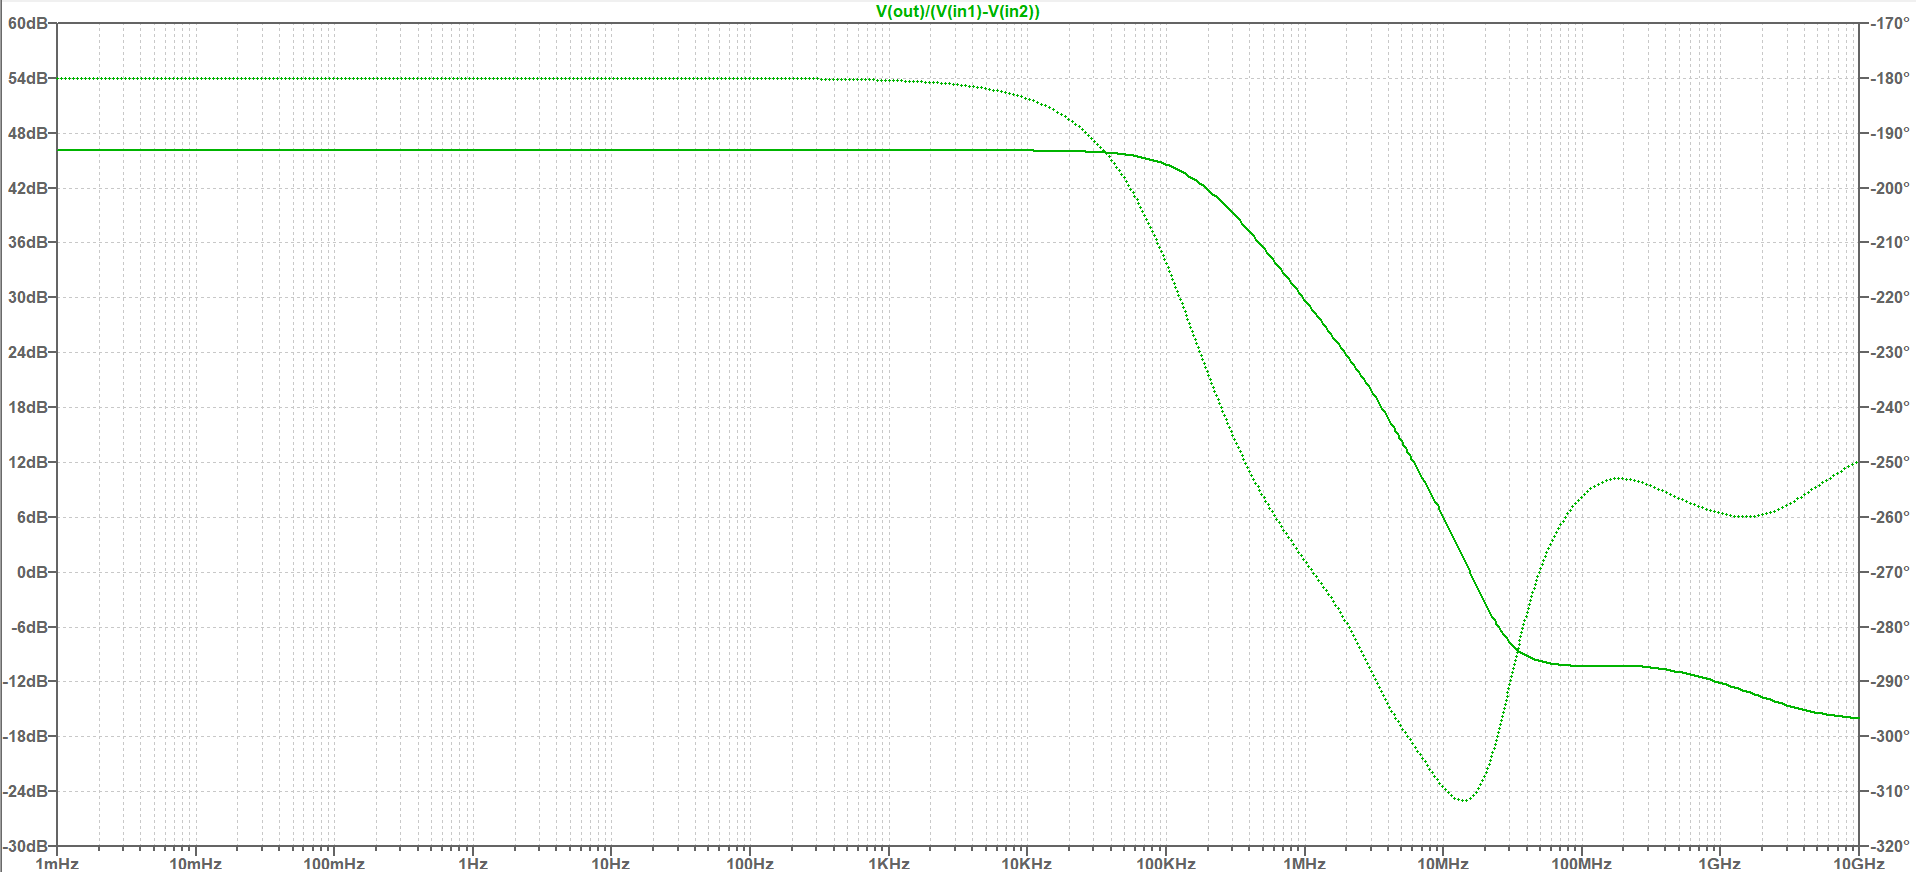
\includegraphics[scale=0.45]{Fig/ac-gain.png}
        \label{fig:ACgain}
        \caption{gain in different frequencies}
    \end{center}
\end{figure}
a) the gain was 46.02dB (200) in theory and is about 46dB also in simulation.(though we made small changes in widlar part in simulation due to errors) \\
b) gain also drops below 3dB at 12.6MHz. \\
c) unity gain bandwidth is at 15.6MHz. \\
d) \\
\begin{figure}[H]
    \begin{center}
        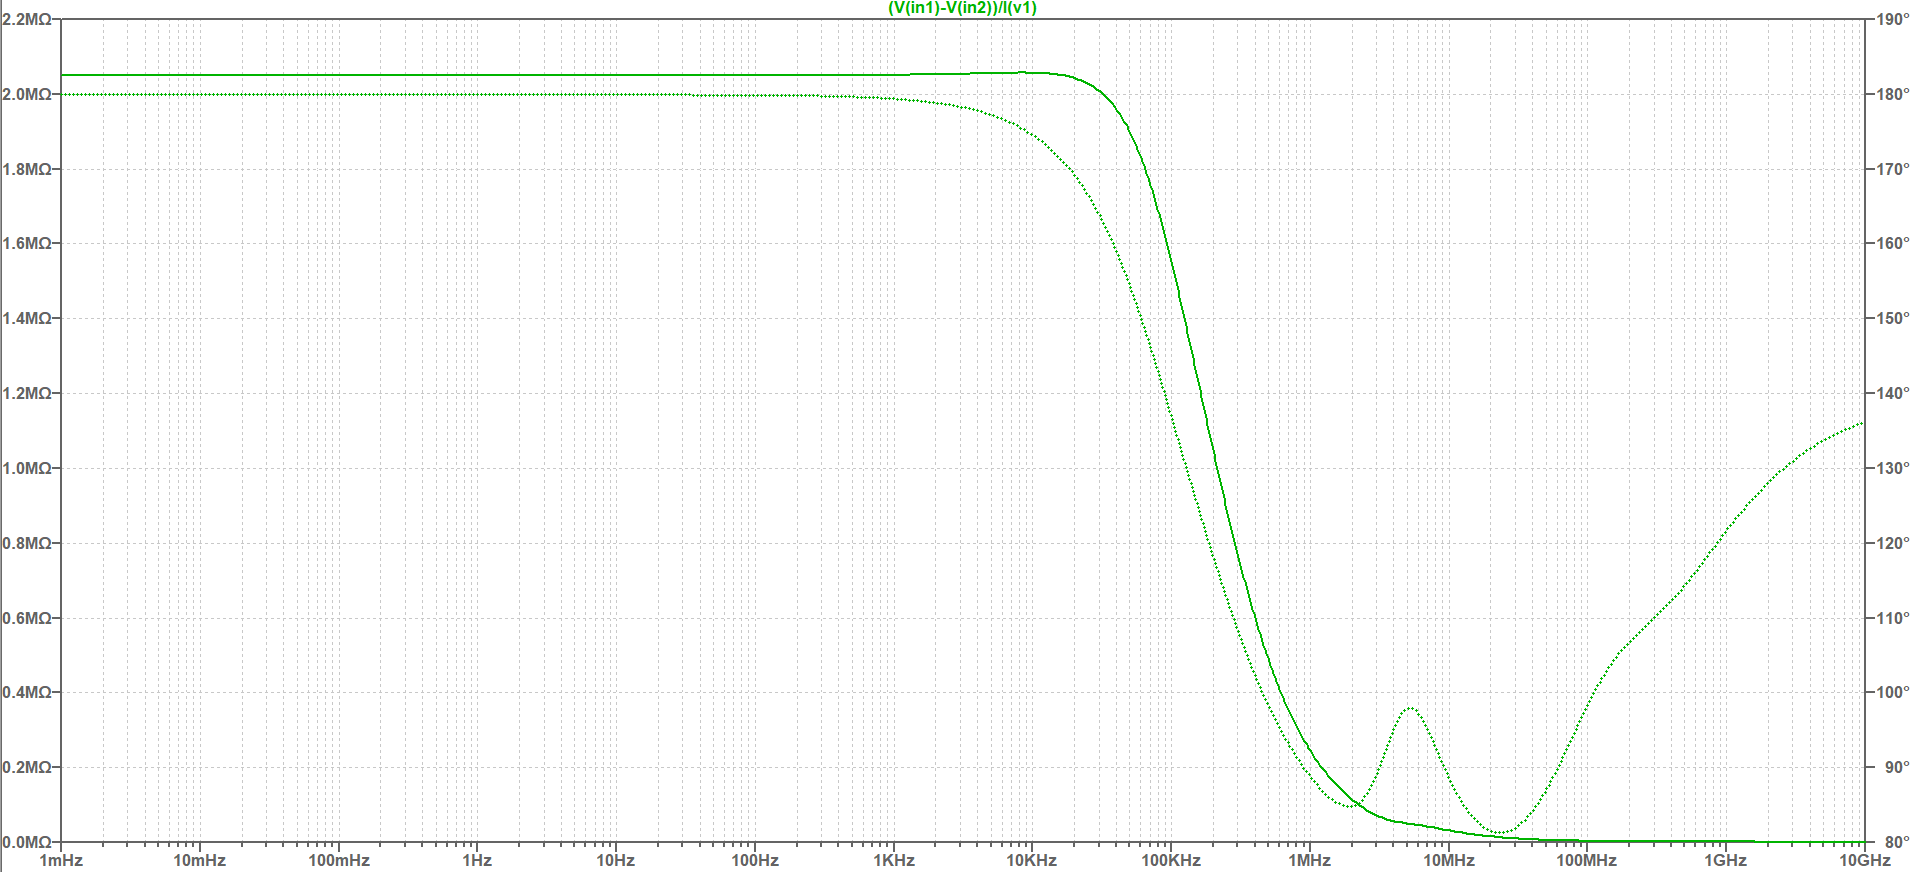
\includegraphics[scale=0.45]{Fig/ac-in-resistance.png}
        \label{fig:ACinResistance}
        \caption{input resistance in different frequencies}
    \end{center}
\end{figure}
\begin{figure}[H]
    \begin{center}
        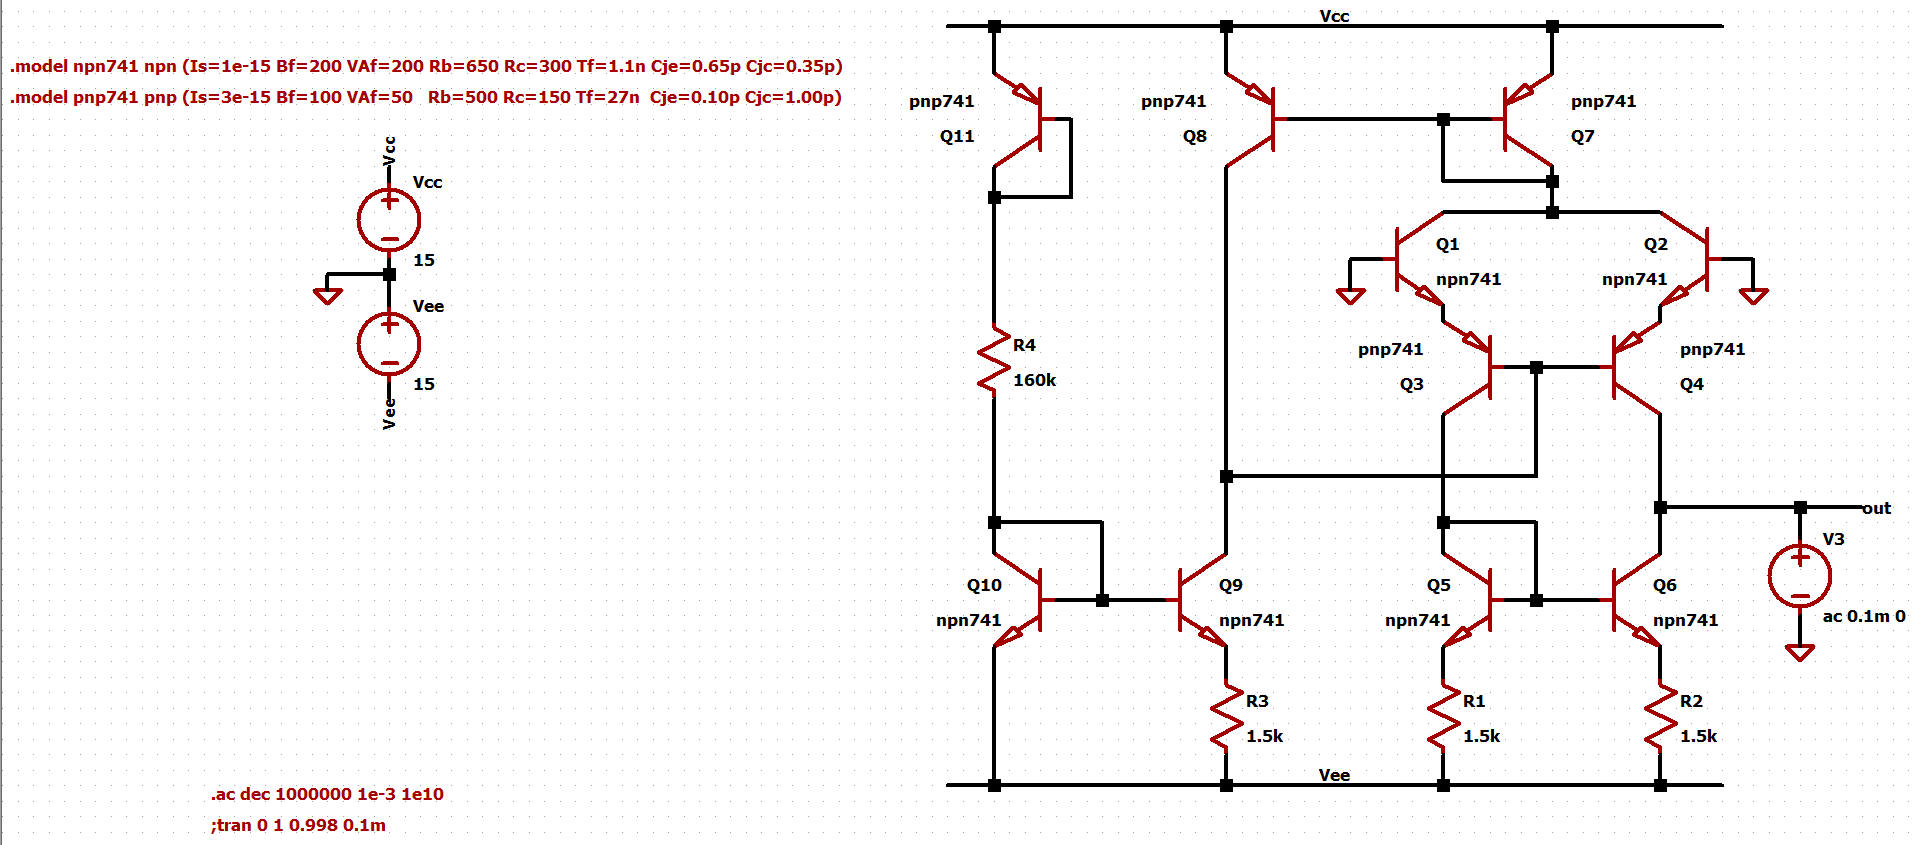
\includegraphics[scale=0.45]{Fig/ac-outR-circuit.png}
        \label{fig:ACoutRCirc}
        \caption{the circuit for seeing output resistance($R_L = \infty$ because it shouldn't be seen in output resistance)}
    \end{center}
\end{figure}
\begin{figure}[H]
    \begin{center}
        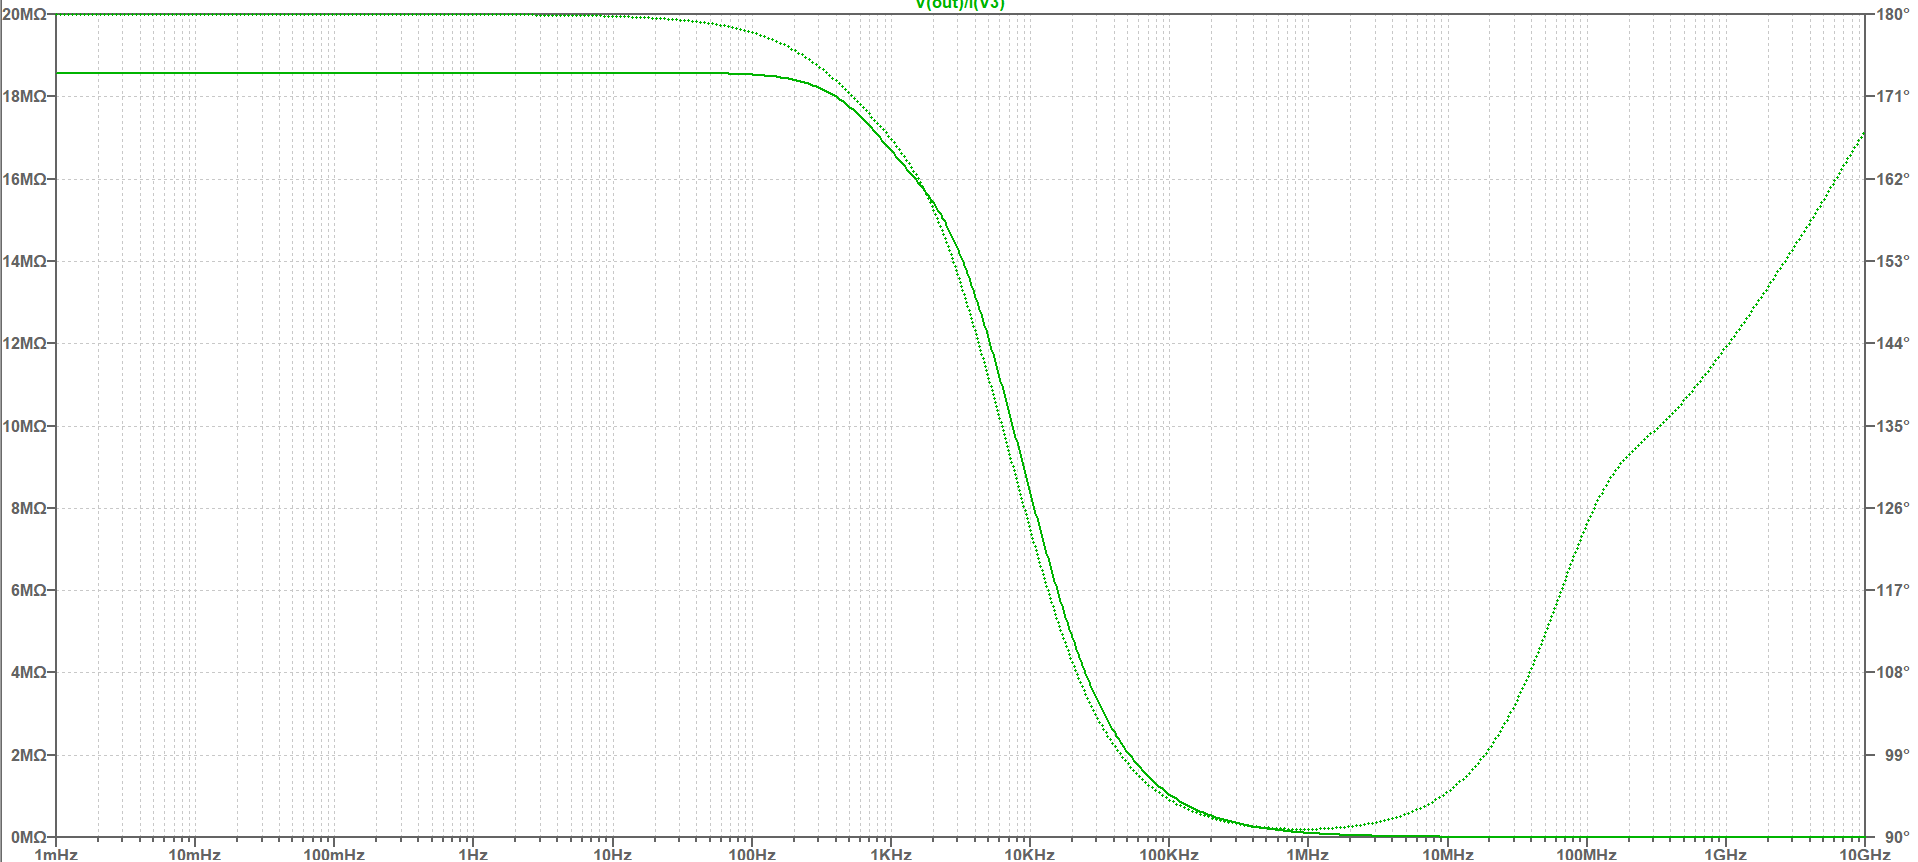
\includegraphics[scale=0.45]{Fig/ac-outR.png}
        \label{fig:ACoutR}
        \caption{output resistance in different frequencies}
    \end{center}
\end{figure}
we can see that: $R_{in} = 2.1M\Omega$ and $R_{out} = 18.6M\Omega$ \\ \\

e) we again do all the above steps:
\begin{figure}[H]
    \begin{center}
        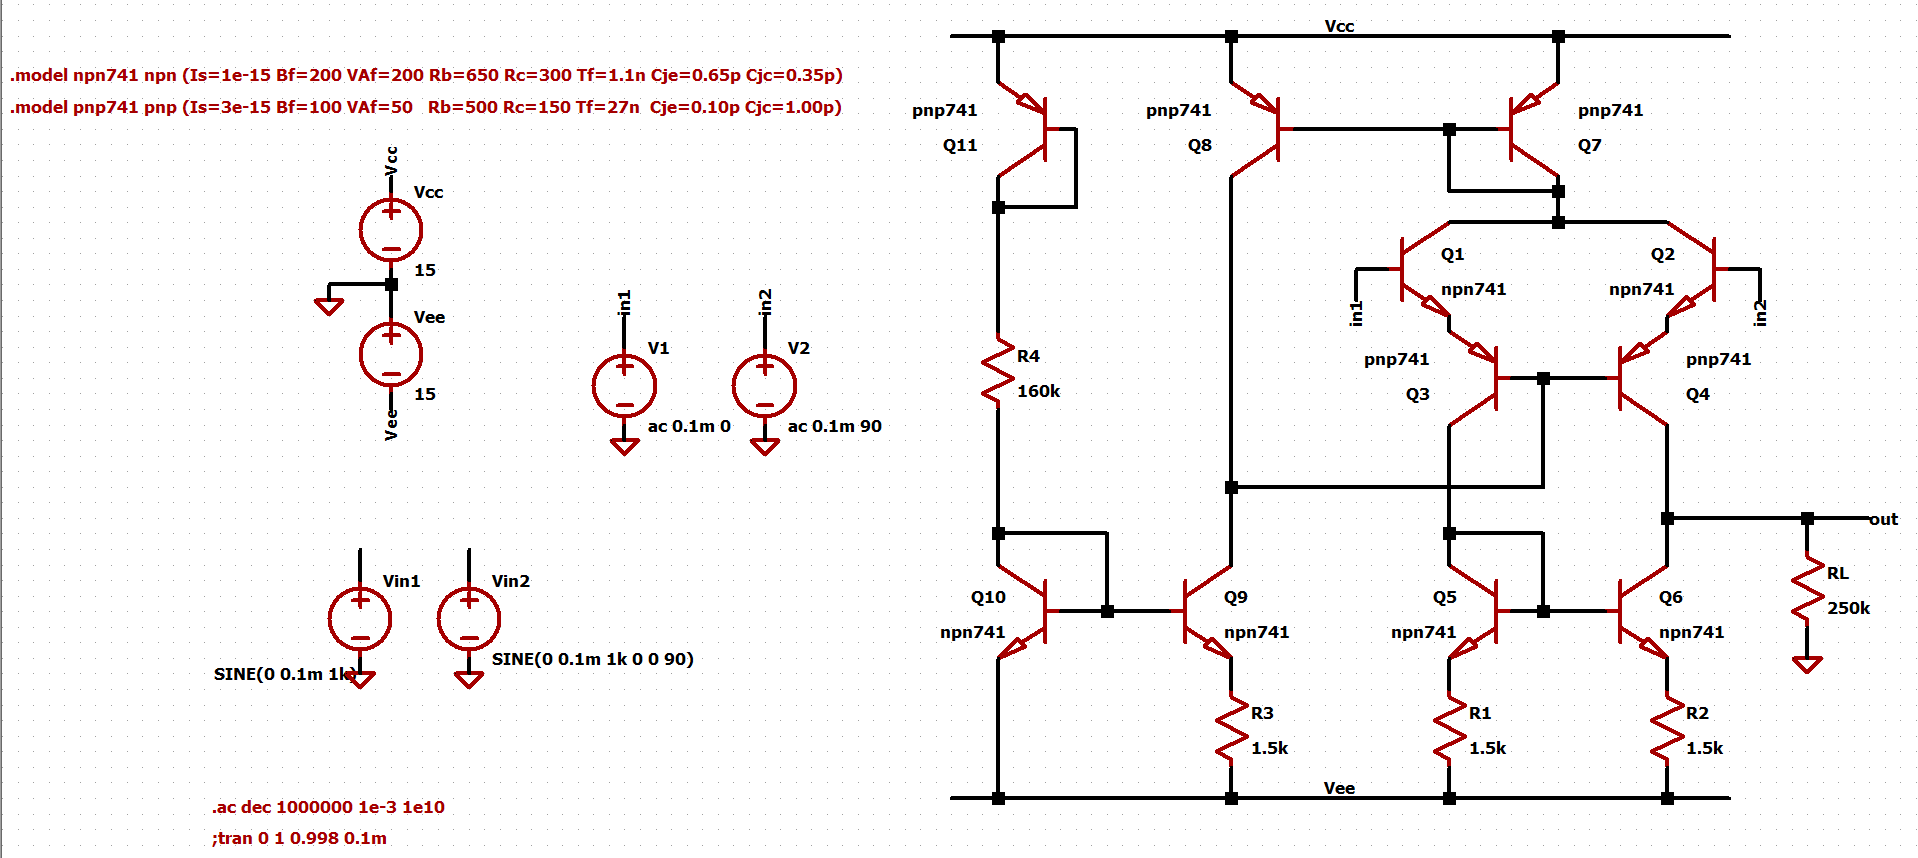
\includegraphics[scale=0.4]{Fig/ac-circuit250.png}
        \label{fig:ACCircuit250}
        \caption{the AC circuit in ltspice(250k)}
    \end{center}
\end{figure}

\begin{figure}[H]
    \begin{center}
        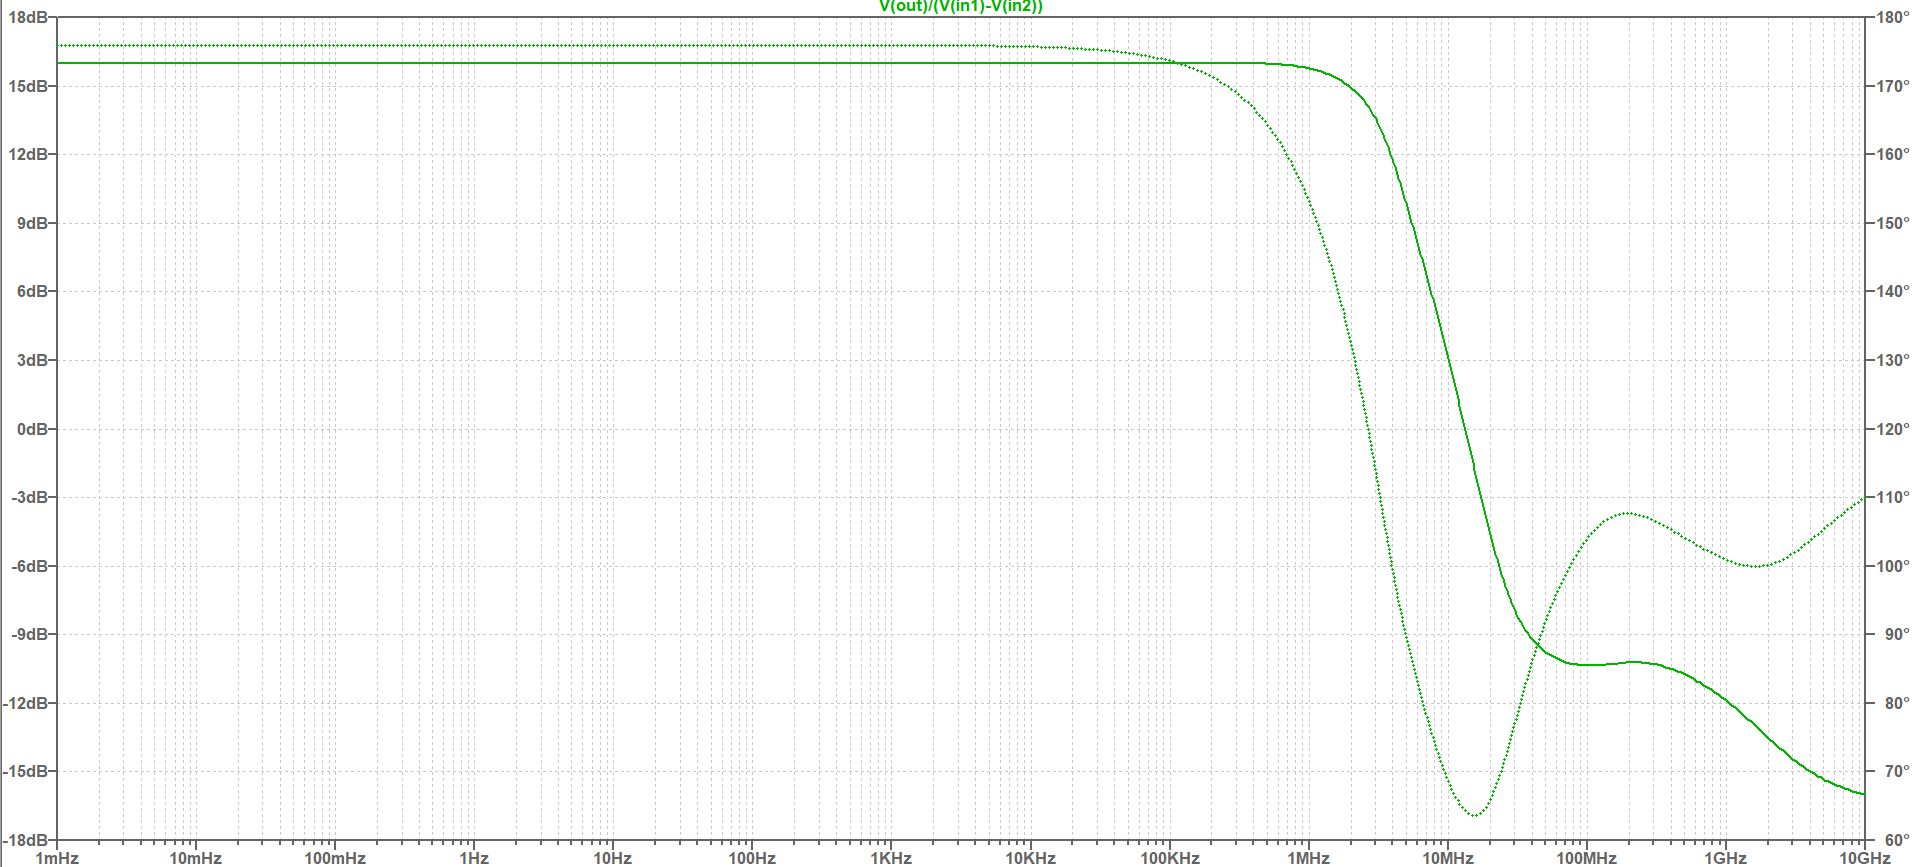
\includegraphics[scale=0.45]{Fig/ac-gain250.png}
        \label{fig:ACgain250}
        \caption{gain in different frequencies(250k)}
    \end{center}
\end{figure}
\begin{figure}[H]
    \begin{center}
        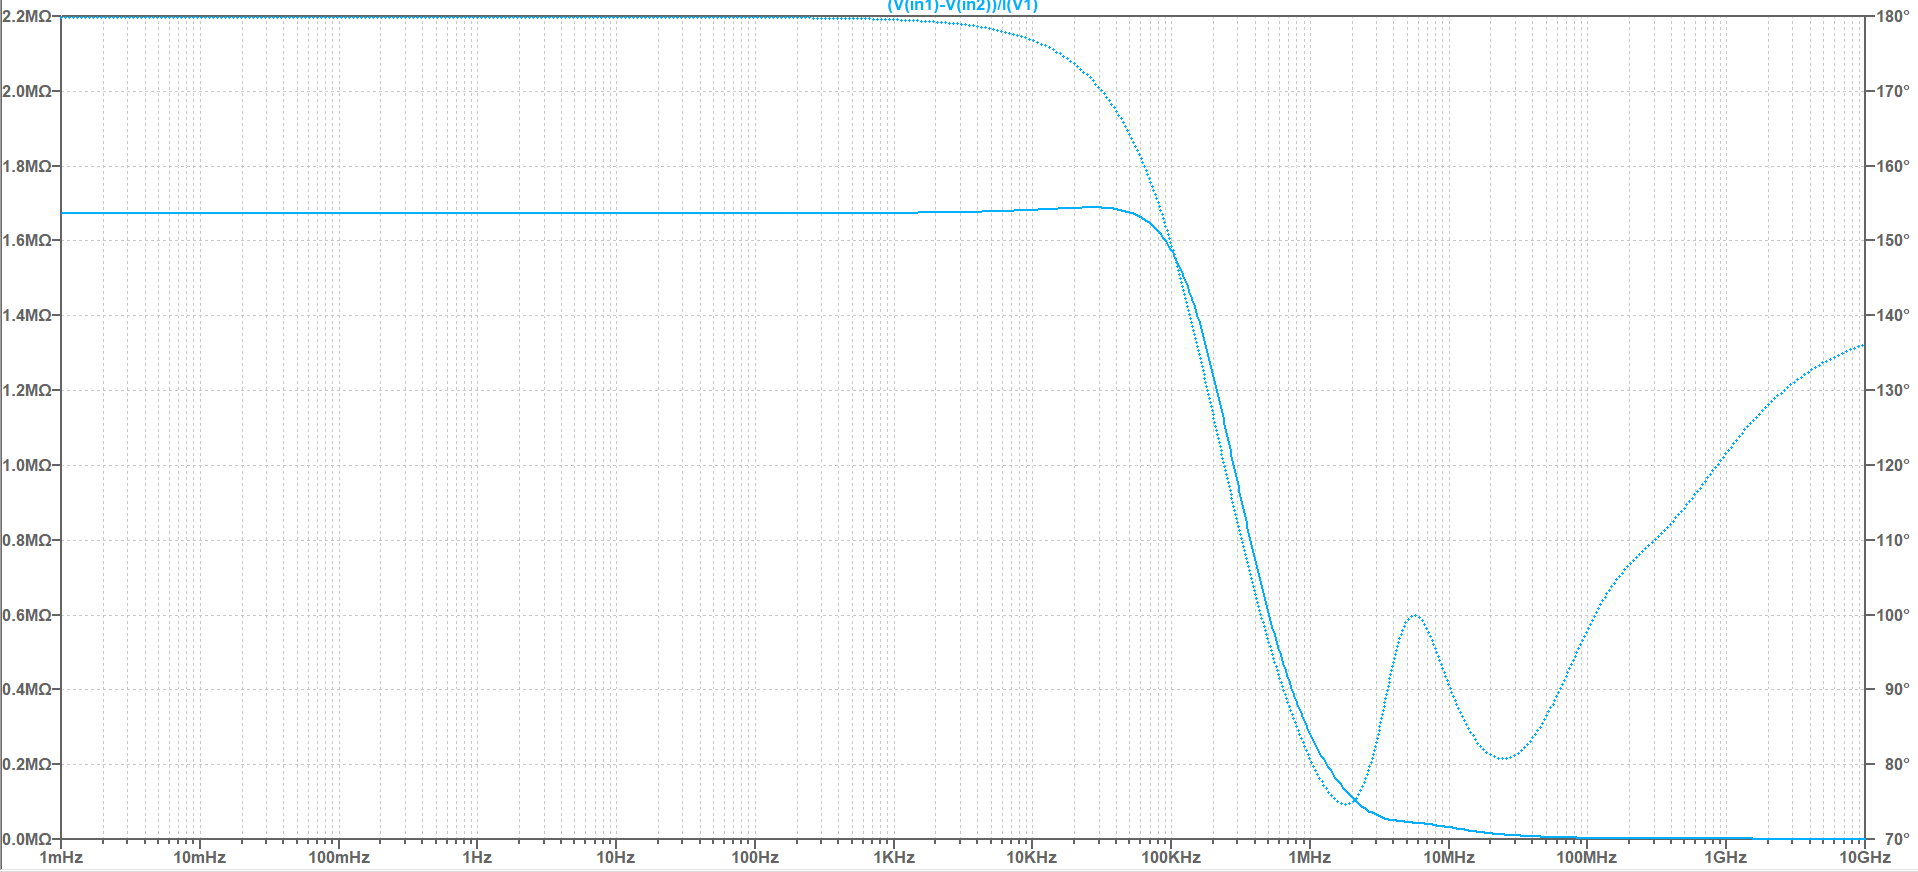
\includegraphics[scale=0.45]{Fig/ac-in-resistance250.png}
        \label{fig:ACinResistance250}
        \caption{input resistance in different frequencies(250k)}
    \end{center}
\end{figure}
the gain is about 16dB. \\
the 3dB gain is at 10MHz. \\
the 0dB gain is 13.3MHz. \\
the input impedance is at 1.7M$\Omega$. \\
the output impedance is the same always regardless of the load so it is again 18.6M$\Omega$.


\subsection{testing the circuit at 1kHz frequency}
a)
\begin{figure}[H]
    \begin{center}
        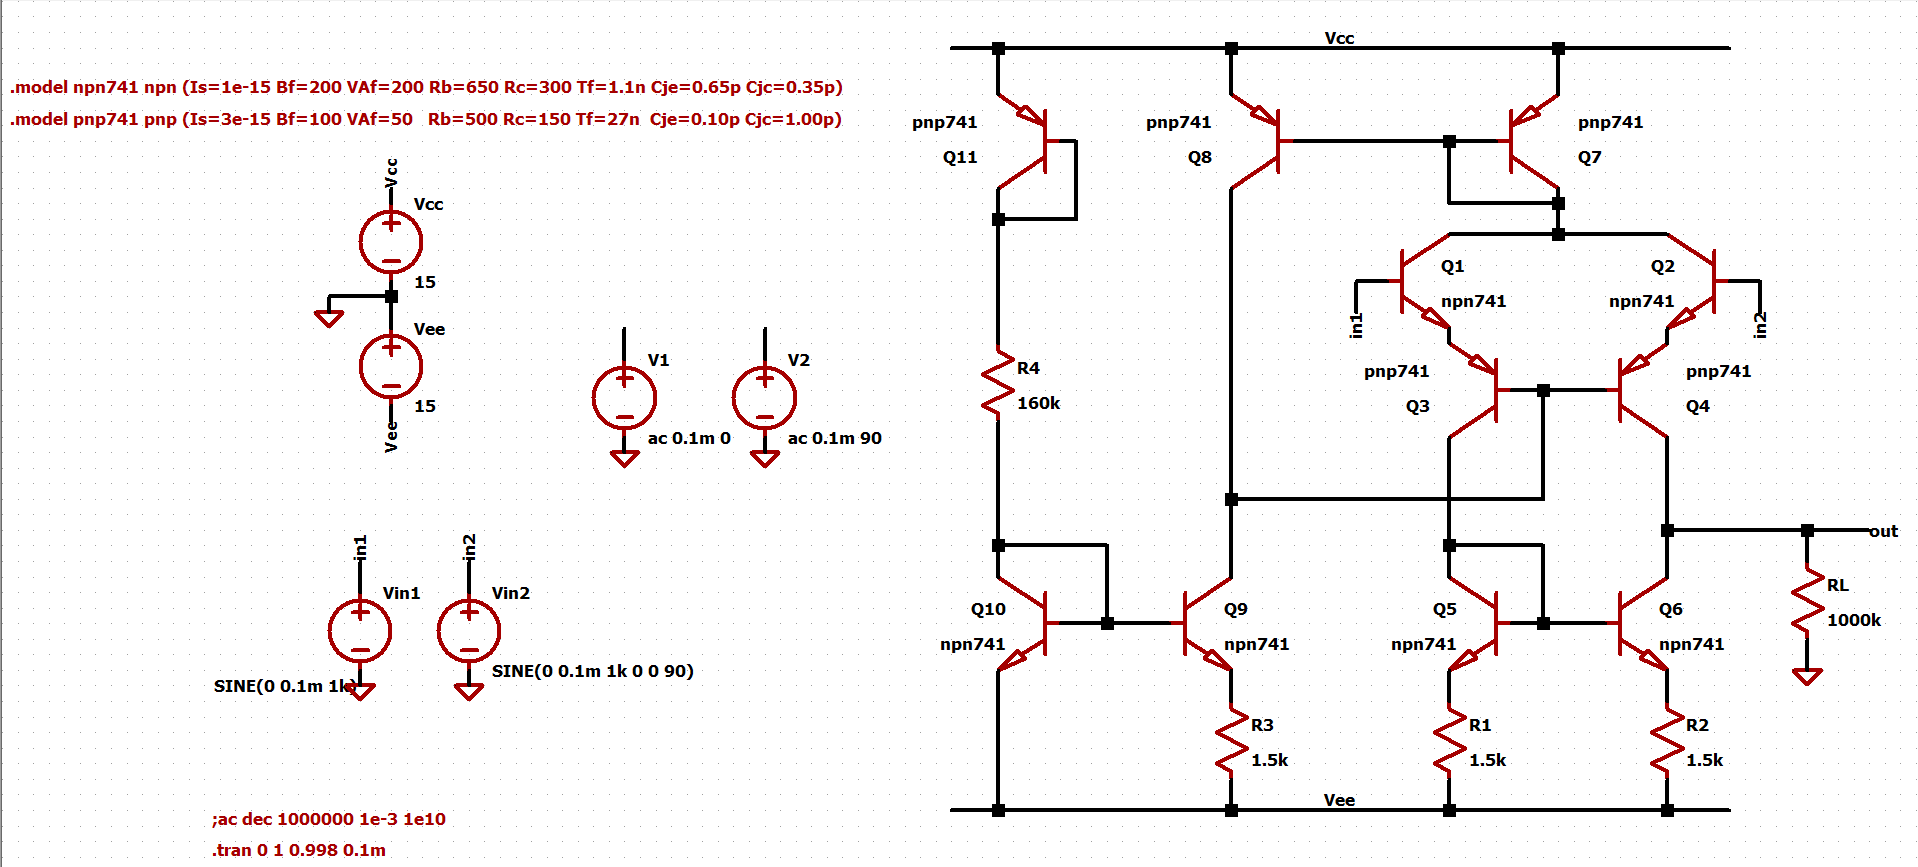
\includegraphics[scale=0.45]{Fig/1k-circuit.png}
        \label{fig:1ktransientCircuit}
        \caption{the circuit in 1k transient}
    \end{center}
\end{figure}

\begin{figure}[H]
    \begin{center}
        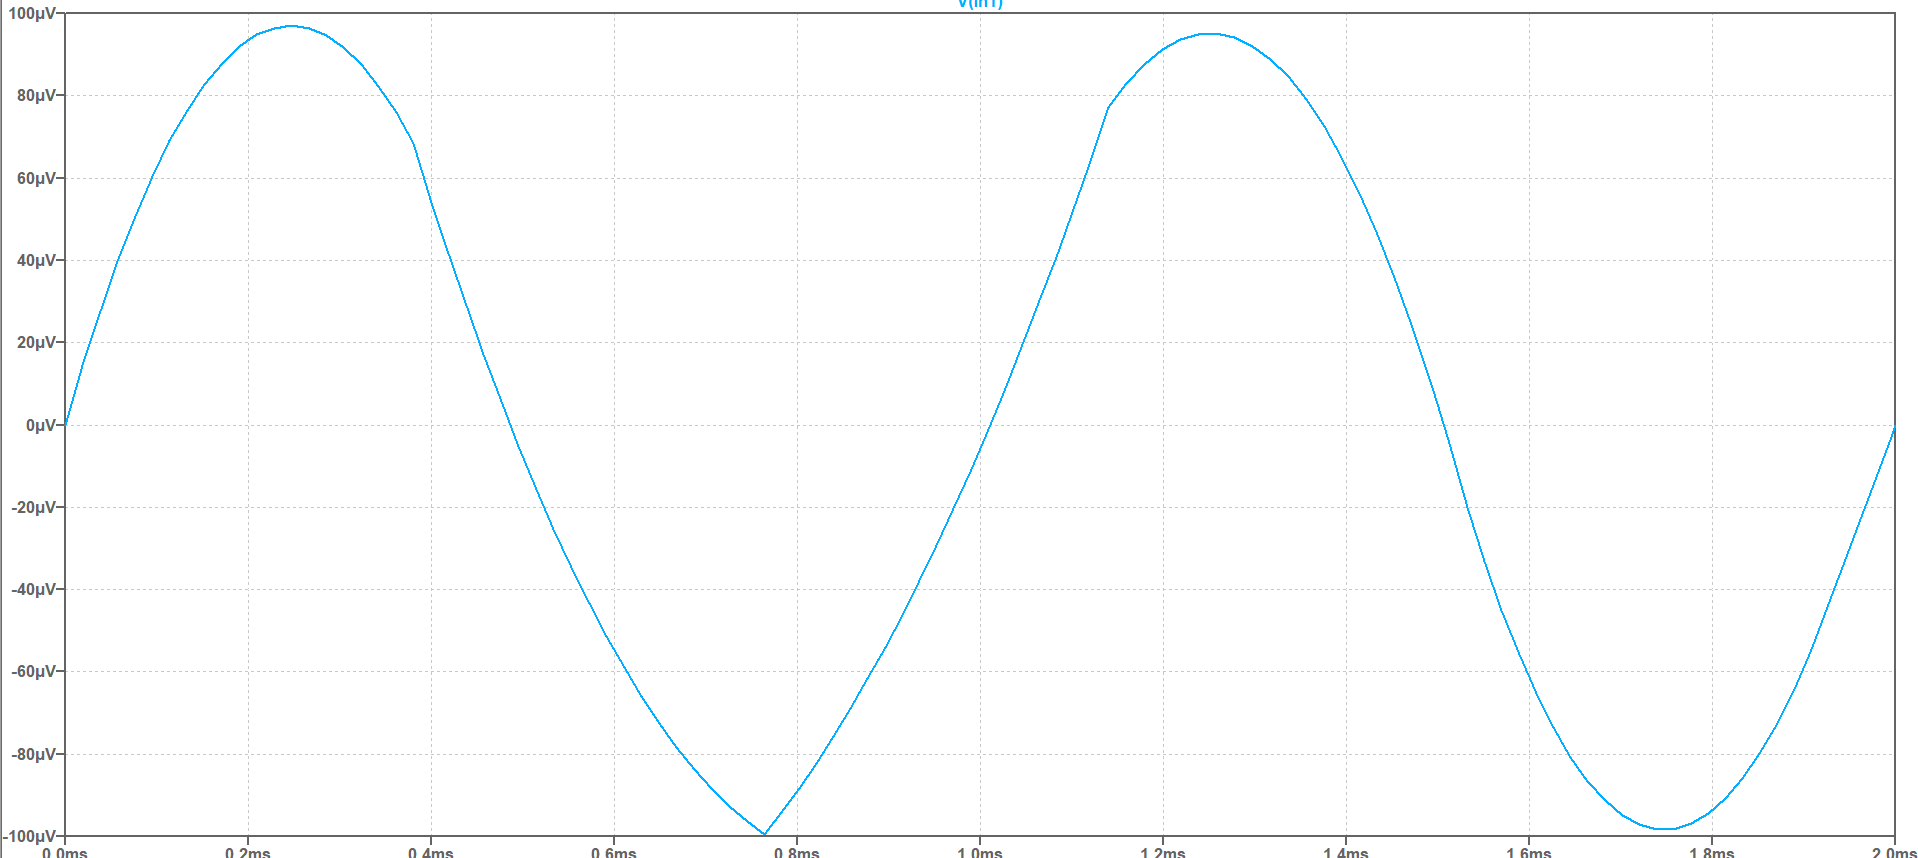
\includegraphics[scale=0.45]{Fig/1k-input.png}
        \label{fig:1kfreqinput}
        \caption{the input(0.1m $v_{in1}$ with 1k frequency)}
    \end{center}
\end{figure}

\begin{figure}[H]
    \begin{center}
        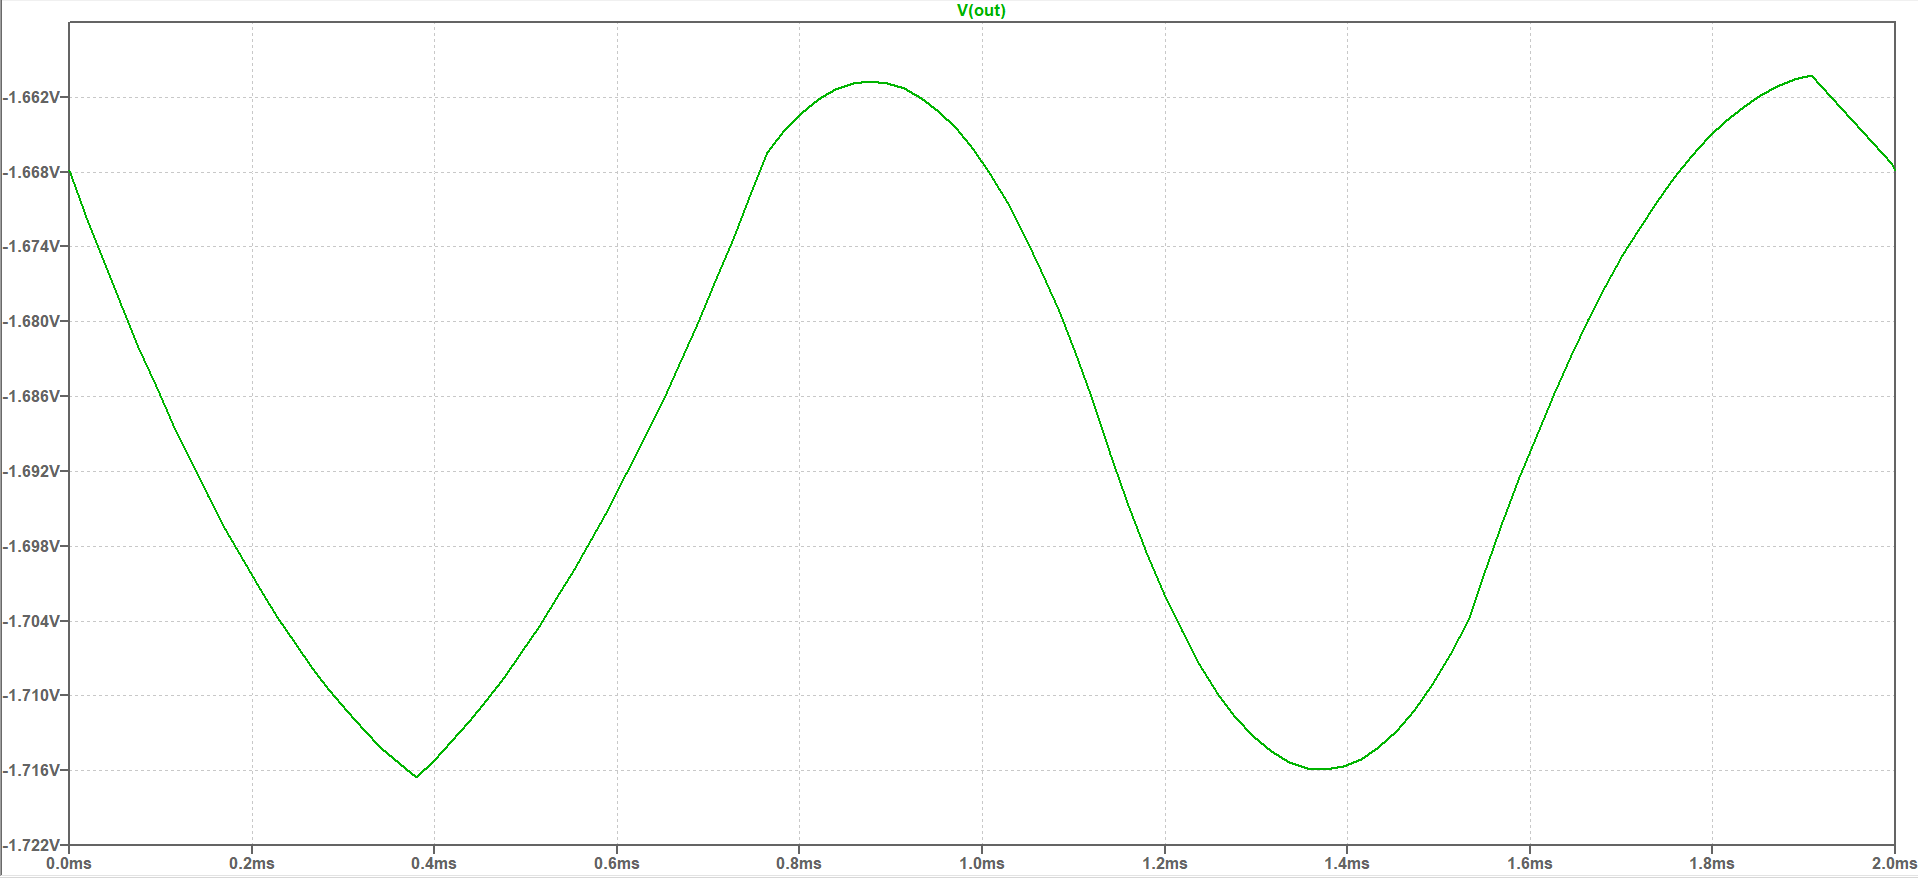
\includegraphics[scale=0.45]{Fig/1k-output.png}
        \label{fig:1kfreqout}
        \caption{the output to the input with 0.2mV amplitude}
    \end{center}
\end{figure}

it can be seen that the gain is 270 wich agrees with the AC analysis. \\ \\

b) it can be seen from the figure below that the max swing is between 0 and -15V:
\begin{figure}[H]
    \begin{center}
        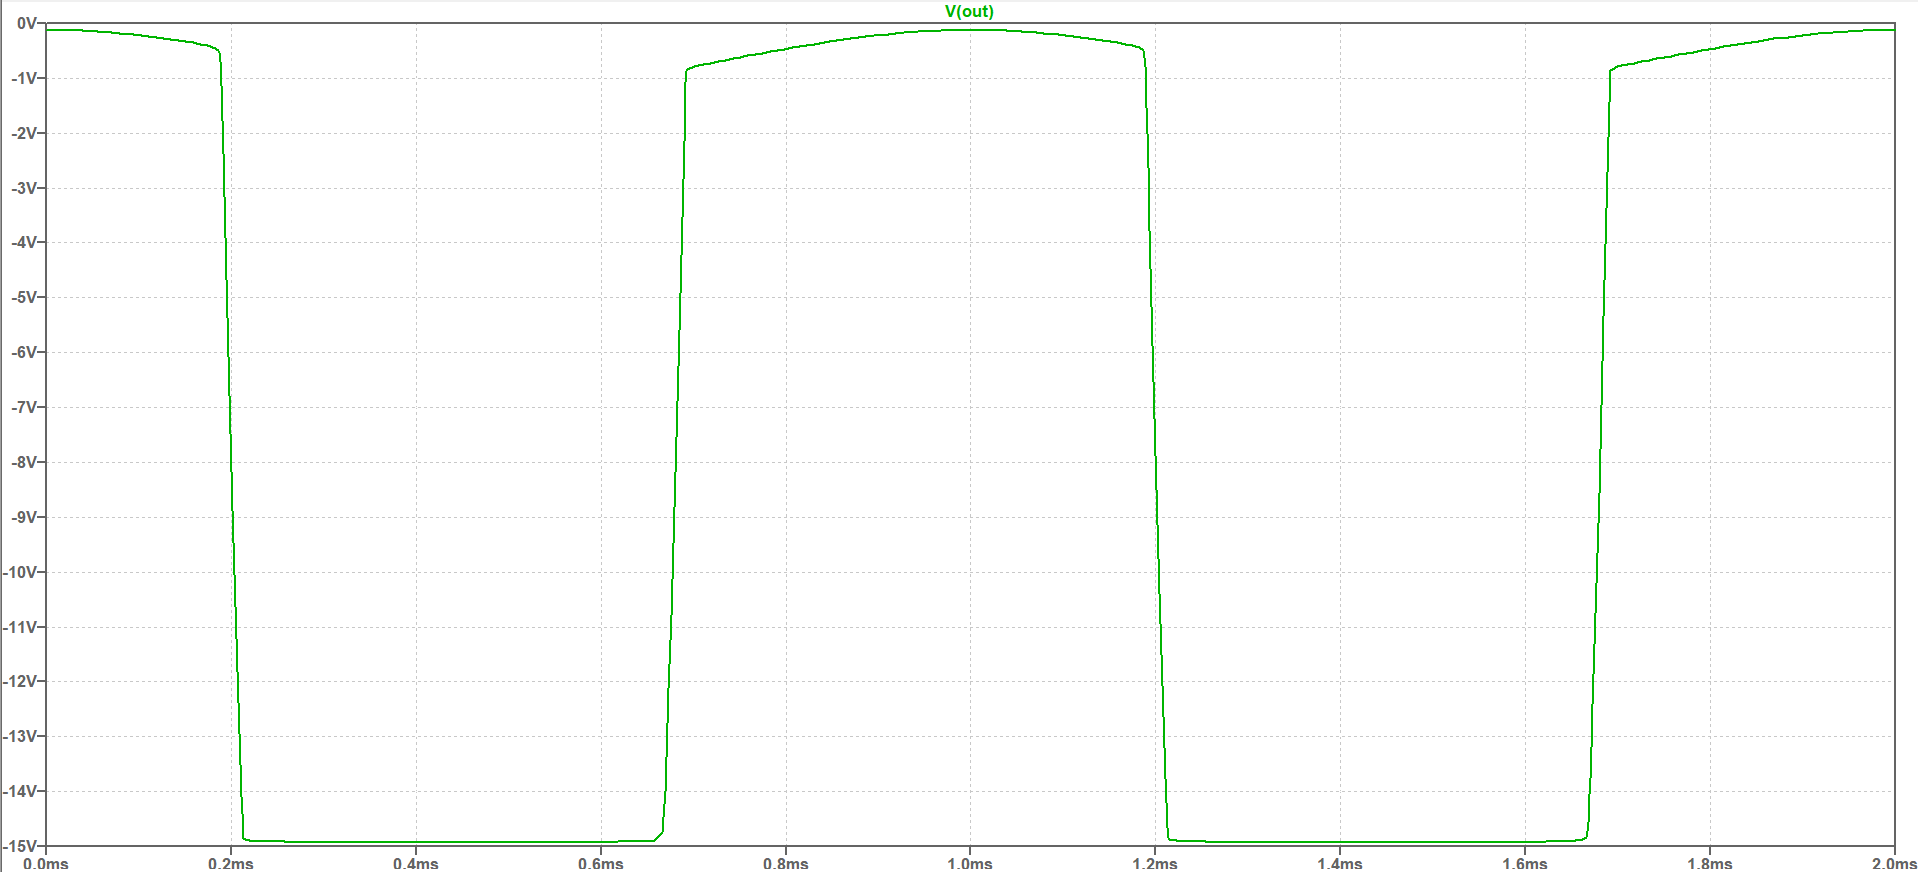
\includegraphics[scale=0.45]{Fig/1k-maxswing.png}
        \label{fig:1kMaxSwing}
        \caption{maximum swing of the circuit(given 500mV input)}
    \end{center}
\end{figure}
c) 
\begin{figure}[H]
    \begin{center}
        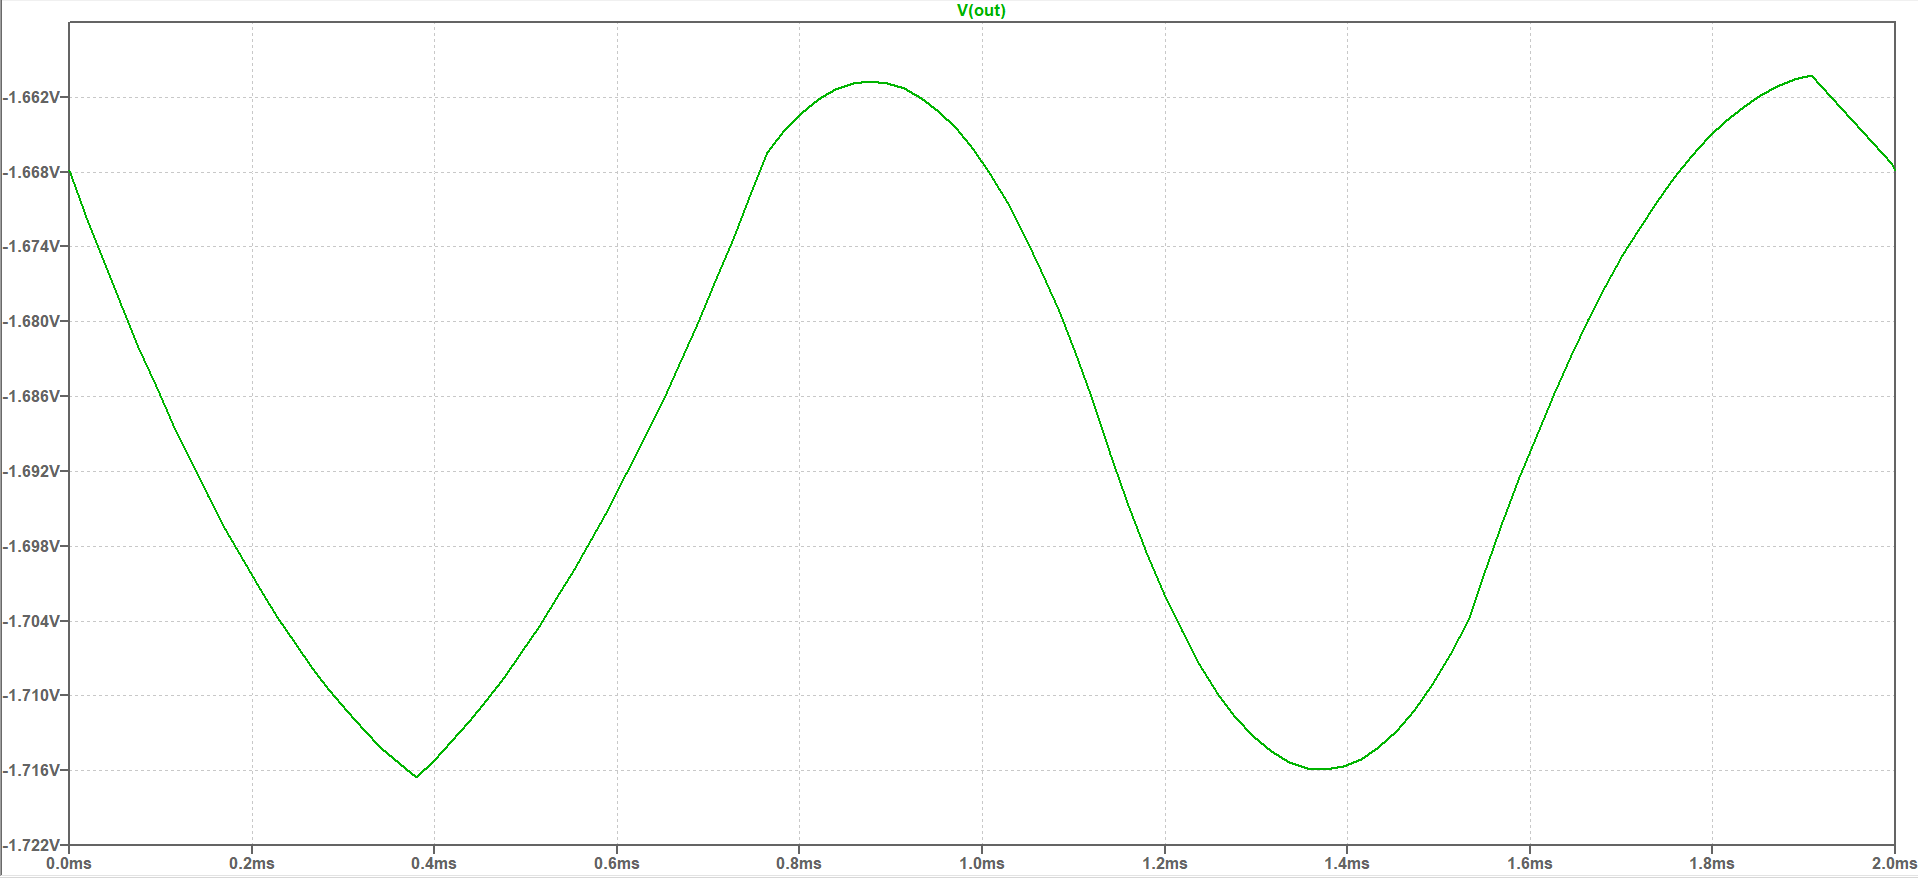
\includegraphics[scale=0.45]{Fig/1k-output.png}
        \label{fig:1kfreqout}
        \caption{the output to the input with 0.2mV amplitude}
    \end{center}
\end{figure}

\begin{figure}[H]
    \begin{center}
        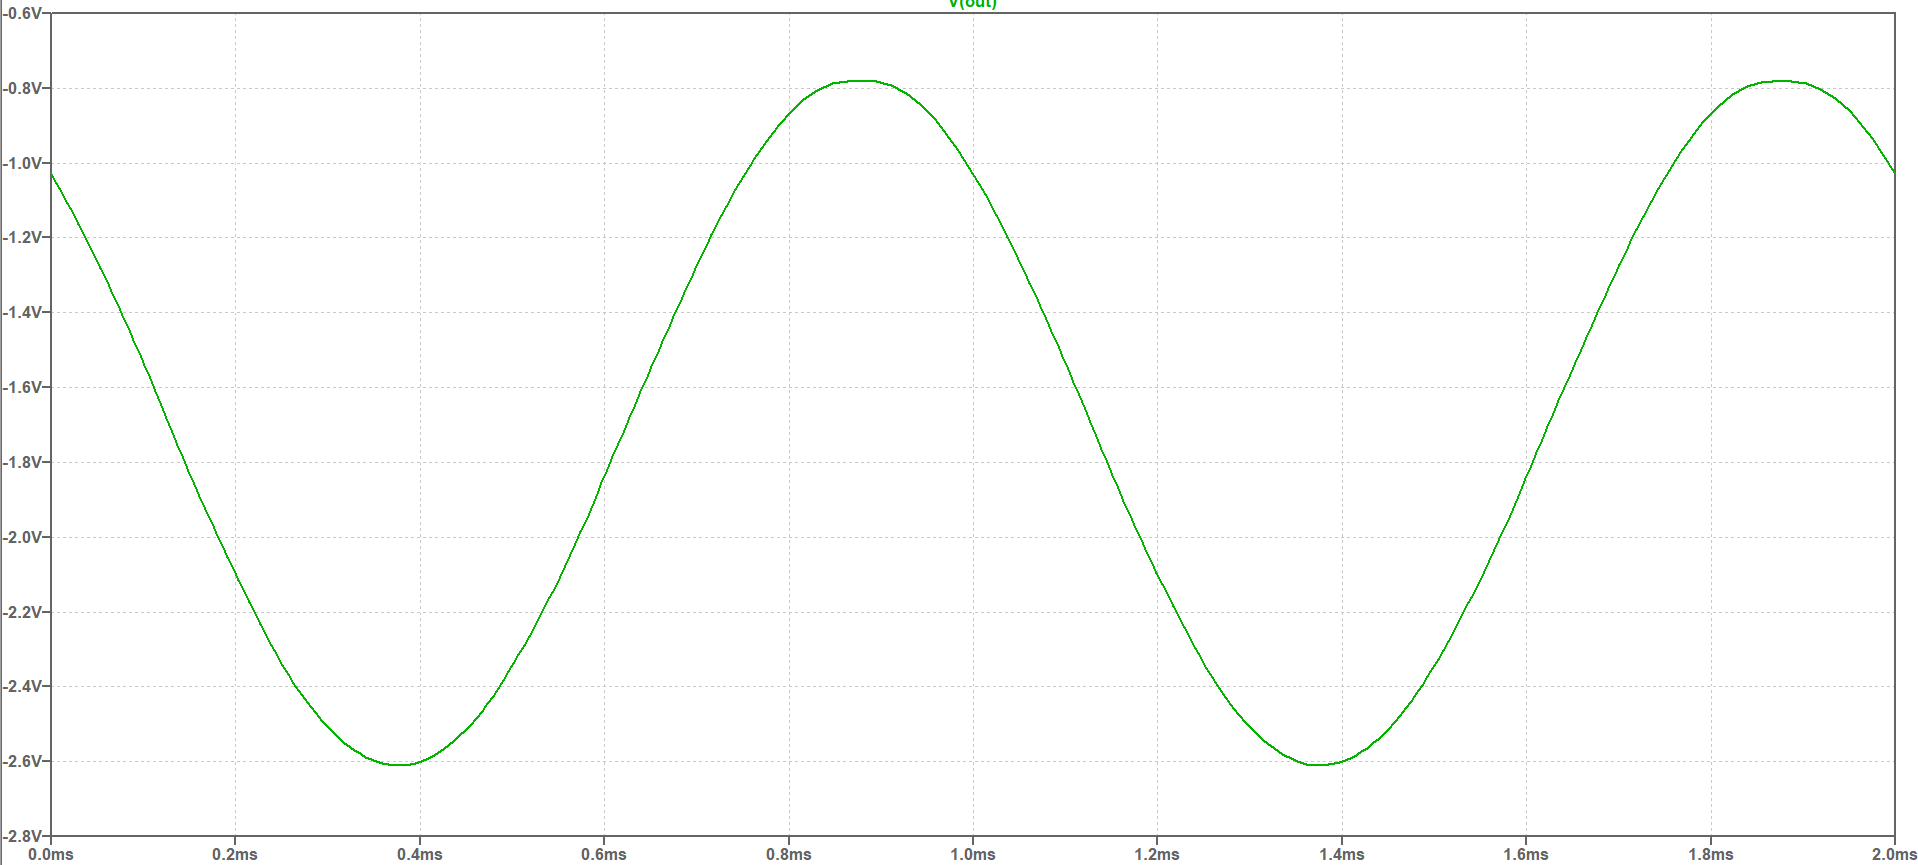
\includegraphics[scale=0.45]{Fig/1k-unlinaer.png}
        \label{fig:1kfreqout}
        \caption{the output to the input with 6.5mV amplitude}
    \end{center}
\end{figure}

d)
\begin{figure}[H]
    \begin{center}
        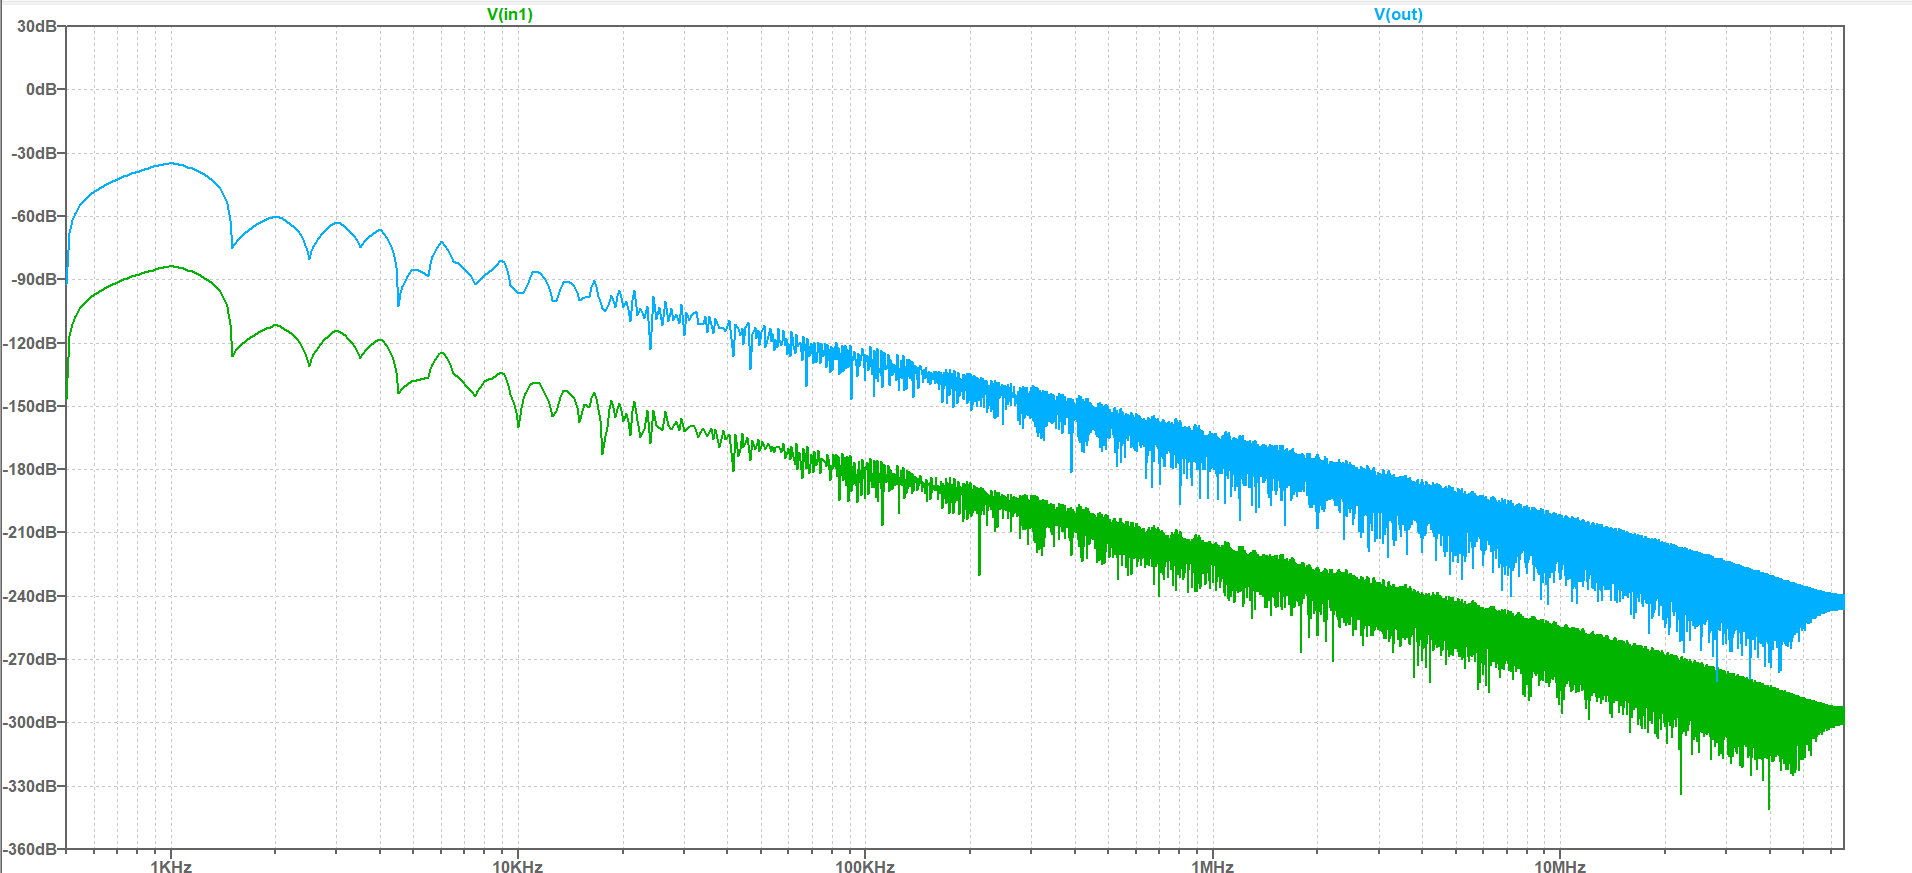
\includegraphics[scale=0.45]{Fig/fourier-linear.png}
        \label{fig:linearFourier}
        \caption{the more linear output fourier}
    \end{center}
\end{figure}

\begin{figure}[H]
    \begin{center}
        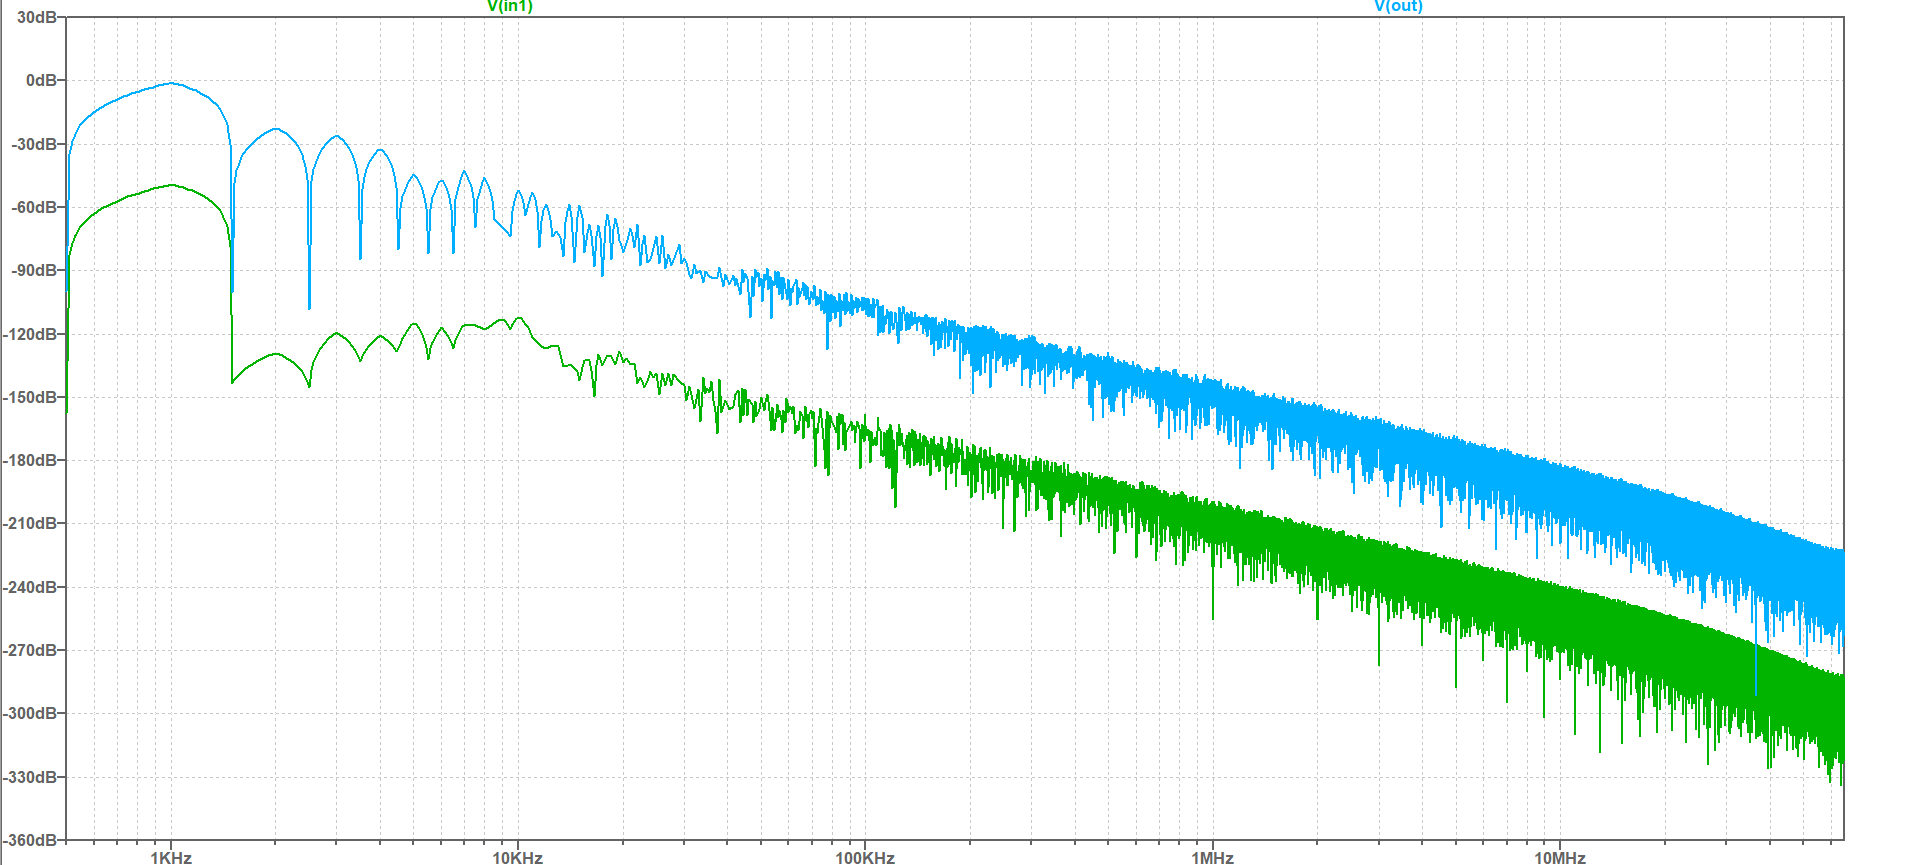
\includegraphics[scale=0.45]{Fig/fourier-non-linear.png}
        \label{fig:nonlinearFourier}
        \caption{the less linear output fourier}
    \end{center}
\end{figure}
but why the fourier transform changes: \\
becaue when the signal is small the transistor work more linear and the calculated slope is
more accurate but as we make the signal larger more terms in the taylor series of transistor characterisitcs
put effect on our signal and change it from the sine wave it was.

\end{document}
